\documentclass[aspectratio=169]{beamer}\usepackage[]{graphicx}\usepackage[]{xcolor}
% maxwidth is the original width if it is less than linewidth
% otherwise use linewidth (to make sure the graphics do not exceed the margin)
\makeatletter
\def\maxwidth{ %
  \ifdim\Gin@nat@width>\linewidth
    \linewidth
  \else
    \Gin@nat@width
  \fi
}
\makeatother

\definecolor{fgcolor}{rgb}{0.345, 0.345, 0.345}
\newcommand{\hlnum}[1]{\textcolor[rgb]{0.686,0.059,0.569}{#1}}%
\newcommand{\hlsng}[1]{\textcolor[rgb]{0.192,0.494,0.8}{#1}}%
\newcommand{\hlcom}[1]{\textcolor[rgb]{0.678,0.584,0.686}{\textit{#1}}}%
\newcommand{\hlopt}[1]{\textcolor[rgb]{0,0,0}{#1}}%
\newcommand{\hldef}[1]{\textcolor[rgb]{0.345,0.345,0.345}{#1}}%
\newcommand{\hlkwa}[1]{\textcolor[rgb]{0.161,0.373,0.58}{\textbf{#1}}}%
\newcommand{\hlkwb}[1]{\textcolor[rgb]{0.69,0.353,0.396}{#1}}%
\newcommand{\hlkwc}[1]{\textcolor[rgb]{0.333,0.667,0.333}{#1}}%
\newcommand{\hlkwd}[1]{\textcolor[rgb]{0.737,0.353,0.396}{\textbf{#1}}}%
\let\hlipl\hlkwb

\usepackage{framed}
\makeatletter
\newenvironment{kframe}{%
 \def\at@end@of@kframe{}%
 \ifinner\ifhmode%
  \def\at@end@of@kframe{\end{minipage}}%
  \begin{minipage}{\columnwidth}%
 \fi\fi%
 \def\FrameCommand##1{\hskip\@totalleftmargin \hskip-\fboxsep
 \colorbox{shadecolor}{##1}\hskip-\fboxsep
     % There is no \\@totalrightmargin, so:
     \hskip-\linewidth \hskip-\@totalleftmargin \hskip\columnwidth}%
 \MakeFramed {\advance\hsize-\width
   \@totalleftmargin\z@ \linewidth\hsize
   \@setminipage}}%
 {\par\unskip\endMakeFramed%
 \at@end@of@kframe}
\makeatother

\definecolor{shadecolor}{rgb}{.97, .97, .97}
\definecolor{messagecolor}{rgb}{0, 0, 0}
\definecolor{warningcolor}{rgb}{1, 0, 1}
\definecolor{errorcolor}{rgb}{1, 0, 0}
\newenvironment{knitrout}{}{} % an empty environment to be redefined in TeX

\usepackage{alltt}



\usetheme{default}
% Slide setup, colour independent

\usepackage{amsmath,amssymb,amsthm}
\usepackage[utf8]{inputenc}
\usepackage{colortbl}
\usepackage{bm}
\usepackage{xcolor}
\usepackage{dsfont}
\usepackage{setspace}
% To use \ding{234} and the like
\usepackage{pifont}
% To cross reference between slide files
\usepackage{zref-xr,zref-user}
% Use something like
% \zexternaldocument{fileI}
% in the tex files. And cite using \zref instead of \ref
\usepackage{booktabs}
\usepackage{marvosym}
\usepackage{cancel}
%\usepackage{transparent}
% Make doi clickable in the bibliography?
\usepackage{doi}

\usepackage[T1]{fontenc}

\usepackage{longtable}

% For heavier titles
\usepackage{helvet} % Enables Helvetica font family


% Fields and the like
\def\IC{\mathbb{C}}
\def\IE{\mathbb{E}}
\def\IF{\mathbb{F}}
\def\II{\mathbb{I}}
\def\IJ{\mathbb{J}}
\def\IK{\mathbb{K}}
\def\IM{\mathbb{M}}
\def\IN{\mathbb{N}}
\def\IP{\mathbb{P}}
\def\IR{\mathbb{R}}
\newcommand{\IRplus}{\mathbb{R}_{\ge 0}}
\def\IZ{\mathbb{Z}}
\def\11{\mathds{1}}


% Bold lowercase
\def\ba{\bm{a}}
\def\bb{\bm{b}}
\def\bc{\bm{c}}
\def\bd{\bm{d}}
\def\be{\bm{e}}
\def\bf{\bm{f}}
\def\bg{\bm{g}}
\def\bh{\bm{h}}
\def\bi{\bm{i}}
\def\bj{\bm{j}}
\def\bk{\bm{k}}
\def\bn{\bm{n}}
\def\bp{\bm{p}}
\def\br{\bm{r}}
\def\bs{\bm{s}}
\def\bu{\bm{u}}
\def\bv{\bm{v}}
\def\bw{\bm{w}}
\def\bx{\bm{x}}
\def\by{\bm{y}}
\def\bz{\bm{z}}
\newcommand{\vect}[1]{\bm{#1}}

% Bold capitals
\def\bB{\bm{B}}
\def\bD{\bm{D}}
\def\bE{\bm{E}}
\def\bF{\bm{F}}
\def\bG{\bm{G}}
\def\bI{\bm{I}}
\def\bL{\bm{L}}
\def\bN{\bm{N}}
\def\bP{\bm{P}}
\def\bR{\bm{R}}
\def\bS{\bm{S}}
\def\bT{\bm{T}}
\def\bX{\bm{X}}

% Bold numbers
\def\b0{\bm{0}}

% Bold greek
\bmdefine{\bmu}{\bm{\mu}}
\def\bphi{\bm{\phi}}
\def\bvarphi{\bm{\varphi}}
\def\bPi{\bm{\Pi}}
\def\bGamma{\bm{\Gamma}}

% Bold red sentence
\def\boldred#1{{\color{red}\textbf{#1}}}
\def\defword#1{{\color{orange}\textbf{#1}}}

% Caligraphic letters
\def\A{\mathcal{A}}
\def\B{\mathcal{B}}
\def\C{\mathcal{C}}
\def\D{\mathcal{D}}
\def\E{\mathcal{E}}
\def\F{\mathcal{F}}
\def\G{\mathcal{G}}
\def\H{\mathcal{H}}
\def\I{\mathcal{I}}
\def\L{\mathcal{L}}
\def\M{\mathcal{M}}
\def\N{\mathcal{N}}
\def\P{\mathcal{P}}
\def\R{\mathcal{R}}
\def\S{\mathcal{S}}
\def\T{\mathcal{T}}
\def\U{\mathcal{U}}
\def\V{\mathcal{V}}

% Adding space for prime (') where needed
\def\pprime{\,'}
% Adding space for star (\star) where needed
\def\pstar{{\,\star}}

% tt font for code
\def\code#1{{\tt #1}}

% i.e., e.g.
\def\eg{\emph{e.g.}}
\def\ie{\emph{i.e.}}


% Operators and special symbols
\def\nbOne{{\mathchoice {\rm 1\mskip-4mu l} {\rm 1\mskip-4mu l}
{\rm 1\mskip-4.5mu l} {\rm 1\mskip-5mu l}}}
\def\cov{\ensuremath{\mathsf{cov}}}
\def\Var{\ensuremath{\mathsf{Var}\ }}
\def\Im{\textrm{Im}\;}
\def\Re{\textrm{Re}\;}
\def\det{\ensuremath{\mathsf{det}}}
\def\diag{\ensuremath{\mathsf{diag}}}
\def\nullspace{\ensuremath{\mathsf{null}}}
\def\nullity{\ensuremath{\mathsf{nullity}}}
\def\rank{\ensuremath{\mathsf{rank}}}
\def\range{\ensuremath{\mathsf{range}}}
\def\sgn{\ensuremath{\mathsf{sgn}}}
\def\Span{\ensuremath{\mathsf{span}}}
\def\tr{\ensuremath{\mathsf{tr}}}
\def\imply{$\Rightarrow$}
\def\restrictTo#1#2{\left.#1\right|_{#2}}
\newcommand{\parallelsum}{\mathbin{\!/\mkern-5mu/\!}}
\def\dsum{\mathop{\displaystyle \sum }}%
\def\dind#1#2{_{\substack{#1\\ #2}}}

\newcommand{\Qmatrix}[1]{%
  \begin{pmatrix}#1\end{pmatrix}%
}

\DeclareMathOperator{\GL}{GL}
\DeclareMathOperator{\Rel}{Re}
\def\Nt#1{\left|\!\left|\!\left|#1\right|\!\right|\!\right|}
\newcommand{\tripbar}{|\! |\! |}



% The beamer bullet (in base colour)
\def\bbullet{\leavevmode\usebeamertemplate{itemize item}\ }

% Theorems and the like
\newtheorem{proposition}[theorem]{Proposition}
\newtheorem{property}[theorem]{Property}
\newtheorem{importantproperty}[theorem]{Property}
\newtheorem{importanttheorem}[theorem]{Theorem}
%\newtheorem{lemma}[theorem]{Lemma}
%\newtheorem{corollary}[theorem]{Corollary}
\newtheorem{remark}[theorem]{Remark}
\setbeamertemplate{theorems}[numbered]
%\setbeamertemplate{theorems}[ams style]

%
%\usecolortheme{orchid}
%\usecolortheme{orchid}

\def\red{\color[rgb]{1,0,0}}
\def\blue{\color[rgb]{0,0,1}}
\def\green{\color[rgb]{0,1,0}}

% Fix skipping lines after items in the bibliography
\setbeamertemplate{bibliography entry title}{}
\setbeamertemplate{bibliography entry location}{}
\setbeamertemplate{bibliography entry note}{}

% Get rid of navigation stuff
\setbeamertemplate{navigation symbols}{}

% Set footline/header line
\setbeamertemplate{footline}
{%
\quad p. \insertpagenumber \quad--\quad \insertsection\vskip2pt
}
% \setbeamertemplate{headline}
% {%
% \quad\insertsection\hfill p. \insertpagenumber\quad\mbox{}\vskip2pt
% }


\makeatletter
\newlength\beamerleftmargin
\setlength\beamerleftmargin{\Gm@lmargin}
\makeatother

% Colours for special pages
\def\extraContent{yellow!20}


%%%%%%%%%%%%%%%%%
\usepackage{tikz}
\usetikzlibrary{shapes,arrows}
\usetikzlibrary{positioning}
\usetikzlibrary{shapes.symbols,shapes.callouts,patterns}
\usetikzlibrary{calc,fit}
\usetikzlibrary{backgrounds}
\usetikzlibrary{decorations.pathmorphing,fit,petri}
\usetikzlibrary{automata}
\usetikzlibrary{fadings}
\usetikzlibrary{patterns,hobby}
\usetikzlibrary{backgrounds,fit,petri}
\usetikzlibrary{tikzmark}

\usepackage{pgfplots}
\pgfplotsset{compat=1.6}
\pgfplotsset{ticks=none}

\usetikzlibrary{decorations.markings}
\usetikzlibrary{arrows.meta}
\tikzset{>=stealth}

% For tikz
\tikzstyle{cloud} = [draw, ellipse,fill=red!20, node distance=0.87cm,
minimum height=2em]
\tikzstyle{line} = [draw, -latex']


%%% For max frame images
\newenvironment{changemargin}[2]{%
\begin{list}{}{%
\setlength{\topsep}{0pt}%
\setlength{\leftmargin}{#1}%
\setlength{\rightmargin}{#2}%
\setlength{\listparindent}{\parindent}%
\setlength{\itemindent}{\parindent}%
\setlength{\parsep}{\parskip}%
}%
\item[]}{\end{list}}


% Make one image take up the entire slide content area in beamer,.:
% centered/centred full-screen image, with title:
% This uses the whole screen except for the 1cm border around it
% all. 128x96mm
\newcommand{\titledFrameImage}[2]{
\begin{frame}{#1}
%\begin{changemargin}{-1cm}{-1cm}
\begin{center}
\includegraphics[width=108mm,height=\textheight,keepaspectratio]{#2}
\end{center}
%\end{changemargin}
\end{frame}
}

% Make one image take up the entire slide content area in beamer.:
% centered/centred full-screen image, no title:
% This uses the whole screen except for the 1cm border around it
% all. 128x96mm
\newcommand{\plainFrameImage}[1]{
\begin{frame}[plain]
%\begin{changemargin}{-1cm}{-1cm}
\begin{center}
\includegraphics[width=108mm,height=76mm,keepaspectratio]{#1}
\end{center}
%\end{changemargin}
\end{frame}
}

% Make one image take up the entire slide area, including borders, in beamer.:
% centered/centred full-screen image, no title:
% This uses the entire whole screen
\newcommand{\maxFrameImage}[1]{
\begin{frame}[plain]
\begin{changemargin}{-1cm}{-1cm}
\begin{center}
\includegraphics[width=\paperwidth,height=\paperheight,keepaspectratio]
{#1}
\end{center}
\end{changemargin}
\end{frame}
}

% This uses the entire whole screen (to include in frame)
\newcommand{\maxFrameImageNoFrame}[1]{
\begin{changemargin}{-1cm}{-1cm}
\begin{center}
\includegraphics[width=\paperwidth,height=0.99\paperheight,keepaspectratio]
{#1}
\end{center}
\end{changemargin}
}

% Make one image take up the entire slide area, including borders, in beamer.:
% centered/centred full-screen image, no title:
% This uses the entire whole screen
\newcommand{\maxFrameImageColor}[2]{
\begin{frame}[plain]
\setbeamercolor{normal text}{bg=#2!20}
\begin{changemargin}{-1cm}{-1cm}
\begin{center}
\includegraphics[width=\paperwidth,height=\paperheight,keepaspectratio]
{#1}
\end{center}
\end{changemargin}
\end{frame}
}


\usepackage{tikz}
\usetikzlibrary{patterns,hobby}
\usepackage{pgfplots}
\pgfplotsset{compat=1.6}
\pgfplotsset{ticks=none}

\usetikzlibrary{backgrounds}
\usetikzlibrary{decorations.markings}
\usetikzlibrary{arrows.meta}
\tikzset{>=stealth}

\tikzset{
  clockwise arrows/.style={
    postaction={
      decorate,
      decoration={
        markings,
        mark=between positions 0.1 and 0.9 step 40pt with {\arrow{>}},
   }}}}


% Beginning of a section
\newcommand{\newSectionSlide}[1]{
\begin{frame}[noframenumbering,plain]
  \begin{tikzpicture}[remember picture,overlay]
    \node[above right,inner sep=0pt,opacity=0.2] at (current page.south west)
    {
        \includegraphics[height=\paperheight,width=\paperwidth]{#1}
    };
  \end{tikzpicture}
  \setbeamercolor{section in toc}{fg=section_page_list_colour}
  \setbeamerfont{section in toc}{size=\Large,series=\bfseries}
  \setbeamertemplate{section in toc shaded}[default][60]
  \tableofcontents[
    currentsection,
    sectionstyle=show/shaded,
    subsectionstyle=show/hide/hide,
    subsubsectionstyle=hide/hide/hide]
\end{frame}
\addtocounter{page}{-1}
}

% Beginning of a section in which we also show subsections
\newcommand{\newSectionWithSubsSlide}[1]{
	\begin{frame}[noframenumbering,plain]
		\begin{tikzpicture}[remember picture,overlay]
			\node[above right,inner sep=0pt,opacity=0.2] at (current page.south west)
			{
				\includegraphics[height=\paperheight,width=\paperwidth]{#1}
			};
		\end{tikzpicture}
		\setbeamercolor{section in toc}{fg=section_page_list_colour}
		\setbeamerfont{section in toc}{size=\Large,series=\bfseries}
		\setbeamertemplate{section in toc shaded}[default][60]
		\tableofcontents[
		currentsection,
		sectionstyle=show/hide,
		subsectionstyle=show/show/hide,
		subsubsectionstyle=hide/hide/hide]
	\end{frame}
	\addtocounter{page}{-1}
}

% Beginning of a subsection
\newcommand{\newSubSectionSlide}[1]{
\begin{frame}[noframenumbering,plain]
  \begin{tikzpicture}[remember picture,overlay]
    \node[above right,inner sep=0pt,opacity=0.2] at (current page.south west)
    {
        \includegraphics[height=\paperheight,width=\paperwidth]{#1}
    };
  \end{tikzpicture}
  \setbeamercolor{section in toc}{fg=subsection_page_list_colour}
  \setbeamerfont{section in toc}{size=\Large,series=\bfseries}
  \setbeamertemplate{section in toc shaded}[default][60]
  \setbeamerfont{subsection in toc}{series=\bfseries}
  \setbeamertemplate{subsection in toc shaded}[default][50]
  \tableofcontents[
    currentsection,
    sectionstyle=show/hide,
    subsectionstyle=show/shaded/hide,
    subsubsectionstyle=hide/hide/hide]
\end{frame}
\addtocounter{page}{-1}
}


% Beginning of a subsubsection
\newcommand{\newSubSubSectionSlide}[1]{
\begin{frame}[noframenumbering,plain]
  \begin{tikzpicture}[remember picture,overlay]
    \node[above right,inner sep=0pt,opacity=0.2] at (current page.south west)
    {
        \includegraphics[height=\paperheight,width=\paperwidth]{#1}
    };
  \end{tikzpicture}
  \setbeamercolor{section in toc}{fg=subsub_header_section}
  \setbeamerfont{section in toc}{size=\Large,series=\bfseries}
  \setbeamertemplate{section in toc shaded}[default][60]
  \setbeamerfont{subsection in toc}{series=\bfseries}
  \setbeamertemplate{subsection in toc shaded}[default][50]
  \setbeamertemplate{subsubsection in toc shaded}[default][50]
  \tableofcontents[
    currentsection,
    sectionstyle=show/hide,
    subsectionstyle=show/hide/hide,
    subsubsectionstyle=show/shaded/hide]
\end{frame}
\addtocounter{page}{-1}
}


   %%%%%%%%%%%
% To have links to parts in the outline
\makeatletter
\AtBeginPart{%
  \addtocontents{toc}{\protect\beamer@partintoc{\the\c@part}{\beamer@partnameshort}{\the\c@page}}%
}
%% number, shortname, page.
\providecommand\beamer@partintoc[3]{%
  \ifnum\c@tocdepth=-1\relax
    % requesting onlyparts.
    \makebox[6em]{Part #1:} \textcolor{green!30!blue}{\hyperlink{#2}{#2}}
    \par
  \fi
}
\define@key{beamertoc}{onlyparts}[]{%
  \c@tocdepth=-1\relax
}
\makeatother%

\newcommand{\nameofthepart}{}
\newcommand{\nupart}[1]%
    {   \part{#1}%
        \renewcommand{\nameofthepart}{#1}%
        {
          \setbeamercolor{background canvas}{bg=orange!50}
          \begin{frame}{#1}%\partpage 
          \hypertarget{\nameofthepart}{}\tableofcontents%
          \end{frame}
        }
    }

% This command creates a title page using TikZ only
\newcommand{\tikztitlepage}[1]{%
\begin{frame}[plain,noframenumbering]
  \begin{tikzpicture}[remember picture,overlay]
    % Background image
    \node[above right,inner sep=0pt,opacity=0.1] 
      at (current page.south west) 
      {\includegraphics[width=\paperwidth,height=\paperheight]{#1}};

    % University logo
    \node[anchor=north east, inner sep=5pt, opacity=0.9] 
      at (current page.north east)
      {
\includegraphics[width=0.2\textwidth]{FIGS-slides-admin/UM-logo-horizontal-CMYK.png}};
    
    % Title
    \node[anchor=center, align=center, 
          font=\fontsize{13}{15}\bfseries\color{UMbrown}, 
          text width=0.9\textwidth] 
          at ([yshift=2cm]current page.center)
          {\inserttitle};

      % Authors
      \node[anchor=center, align=center,
        font=\fontsize{10}{12}\bfseries\color{UMbrown},
        text width=0.7\textwidth]
        at ([yshift=0.8cm]current page.center)
        {\insertauthor};

      % Affiliation
      \node[anchor=north, align=center,
        font=\fontsize{9}{11}\color{UMbrown},
        text width=0.7\textwidth]
        at ([yshift=-0.2cm]current page.center)
        {\insertaffiliation};      
    % Date
    \node[anchor=north, align=center, 
          font=\fontsize{12}{16}\bfseries\color{UMbrown},
          text width=0.7\textwidth] 
          at ([yshift=0.2cm]current page.center)
          {\insertdate};

    % Land acknowledgement
    \node[anchor=south, align=justify, 
          font=\footnotesize, text=black, 
          text width=1.1\textwidth] 
          at ([yshift=0.5cm]current page.south)
          {The University of Manitoba campuses are located on original lands of Anishinaabeg, Ininew, Anisininew, Dakota and Dene peoples, and on the National Homeland of the Red River Métis.\\
          We respect the Treaties that were made on these territories, we acknowledge the harms and mistakes of the past, and we dedicate ourselves to move forward in partnership with Indigenous communities in a spirit of Reconciliation and collaboration.};
  \end{tikzpicture}
  \addtocounter{page}{-1}
\end{frame}
}
% The title page with figure
% \newcommand{\titlepagewithfigure}[1]{%
%   \begin{frame}[noframenumbering,plain]
%     \begin{tikzpicture}[remember picture,overlay]
%       \node[above right,inner sep=0pt,opacity=0.1] at (current page.south west)
%       {
%           \includegraphics[height=\paperheight,width=\paperwidth]{#1}
%       };
%       \node[anchor=north east,
%       inner sep=5pt,
%       opacity=0.9] at (current page.north east)
%       {
%           
\includegraphics[width=0.2\textwidth]{FIGS-slides-admin/UM-logo-horizontal-CMYK.png}
%       };
%       \node[anchor=south, 
%       align=justify, 
%       text=black, 
%       text width=1.1\textwidth,
%       font=\footnotesize]  (land_acknowledgement)
%       at (current page.south) 
%       {The University of Manitoba campuses are located on original lands of Anishinaabeg, Ininew, Anisininew, Dakota and Dene peoples, and on the National Homeland of the Red River Métis.
%       We respect the Treaties that were made on these territories, we acknowledge the harms and mistakes of the past, and we dedicate ourselves to move forward in partnership with Indigenous communities in a spirit of Reconciliation and collaboration.};  
%       % \node[align=center, anchor=south,
%       % above=0.5cm of land_acknowledgement,
%       % text=black,
%       % font=\bfseries] {\insertdate};
%   \end{tikzpicture}
%   \setbeamercolor{title}{fg=title_page_title_colour}
%   \setbeamerfont{title}{size=\Large,series=\bfseries}
%   \setbeamercolor{author}{fg=title_page_author_colour}
%   \setbeamerfont{author}{size=\large,series=\bfseries}
%   \setbeamercolor{institute}{fg=title_page_institute_colour}
%   \setbeamerfont{institute}{size=\large,series=\bfseries}
%   \setbeamercolor{date}{fg=title_page_date_colour}
%   \setbeamerfont{date}{series=\bfseries}
% 	\titlepage
% \end{frame}
% \addtocounter{page}{-1}
% }

\newcommand{\titlepagewithfigure}[1]{%
  \begin{frame}[noframenumbering,plain]
    \begin{tikzpicture}[remember picture,overlay]
      \node[above right,inner sep=0pt,opacity=0.1] at (current page.south west)
      {
          \includegraphics[height=\paperheight,width=\paperwidth]{#1}
      };
      \node[anchor=north east,
      inner sep=5pt,
      opacity=0.9] at (current page.north east)
      {
          
\includegraphics[width=0.2\textwidth]{FIGS-slides-admin/UM-logo-horizontal-CMYK.png}
      };
      \node[anchor=south, 
      align=justify, 
      text=black, 
      text width=1.1\textwidth,
      font=\footnotesize]  (land_acknowledgement)
      at (current page.south) 
      {The University of Manitoba campuses are located on original lands of Anishinaabeg, Ininew, Anisininew, Dakota and Dene peoples, and on the National Homeland of the Red River Métis.
      We respect the Treaties that were made on these territories, we acknowledge the harms and mistakes of the past, and we dedicate ourselves to move forward in partnership with Indigenous communities in a spirit of Reconciliation and collaboration.};  
      % \node[align=center, anchor=south,
      % above=0.5cm of land_acknowledgement,
      % text=black,
      % font=\bfseries] {\insertdate};
  \end{tikzpicture}
  \setbeamercolor{title}{fg=title_page_title_colour}
  \setbeamerfont{title}{size=\Large,series=\bfseries,family=\usefont{T1}{phv}{b}{n}}
  \setbeamercolor{author}{fg=title_page_author_colour}
  \setbeamerfont{author}{size=\large,series=\bfseries,family=\usefont{T1}{phv}{b}{n}}
  \setbeamercolor{institute}{fg=title_page_institute_colour}
  \setbeamerfont{institute}{size=\large,series=\bfseries,family=\usefont{T1}{phv}{b}{n}}
  \setbeamercolor{date}{fg=title_page_date_colour}
  \setbeamerfont{date}{series=\bfseries,family=\usefont{T1}{phv}{b}{n}}
	\titlepage
\end{frame}
\addtocounter{page}{-1}
}
% The outline page, with figure
% \newcommand{\outlinepage}[1]{%
% \begin{frame}[noframenumbering,plain]
%   \begin{tikzpicture}[remember picture,overlay]
%     \node[above right,inner sep=0pt,opacity=0.2] at (current page.south west)
%     {
%         \includegraphics[height=\paperheight,width=\paperwidth]{#1}
%     };
%   \end{tikzpicture}
%   \setbeamercolor{section in toc}{fg=outline_page_list_colour}
%   \setbeamerfont{section in toc}{size=\Large,series=\bfseries,family=\sffamily}
%   \frametitle{\textcolor{outline_page_title_colour}{\LARGE\bfseries Outline}}
%   \tableofcontents[hideallsubsections]
% \end{frame}
% \addtocounter{page}{-1}
% }
% The outline page, with figure
\newcommand{\outlinepage}[1]{%
\begin{frame}[noframenumbering,plain]
  \begin{tikzpicture}[remember picture,overlay]
    \node[above right,inner sep=0pt,opacity=0.2] at (current page.south west)
    {
        \includegraphics[height=\paperheight,width=\paperwidth]{#1}
    };
  \end{tikzpicture}
  \setbeamercolor{section in toc}{fg=outline_page_list_colour}
  % Use Helvetica Bold only for the outline slide TOC
  \setbeamerfont{section in toc}{size=\Large,family=\usefont{T1}{phv}{b}{n}}
  % Use Helvetica Bold for the outline title
  \frametitle{\textcolor{outline_page_title_colour}{\usefont{T1}{phv}{b}{n}\LARGE Outline}}
  \tableofcontents[hideallsubsections]
\end{frame}
\addtocounter{page}{-1}
}


%\let\oldsection\section
%\renewcommand{\section}[2]{\oldsection[#1]\newSectionSlide[#2]}





\usecolortheme{orchid}
%% Listings
\usepackage{listings}
\definecolor{mygreen}{rgb}{0,0.6,0}
\definecolor{mygray}{rgb}{0.5,0.5,0.5}
\definecolor{mymauve}{rgb}{0.58,0,0.82}
\definecolor{mygold}{rgb}{1,0.843,0}
\definecolor{myblue}{rgb}{0.537,0.812,0.941}

\definecolor{mygold2}{RGB}{120,105,22}
\definecolor{mygrey2}{RGB}{50,50,50}

\definecolor{lgreen}{rgb}{0.6,0.9,.6}
\definecolor{lred}{rgb}{1,0.5,.5}

\lstloadlanguages{R}
\lstset{ %
  language=R,
  backgroundcolor=\color{black!05},   % choose the background color
  basicstyle=\footnotesize\ttfamily,        % size of fonts used for the code
  breaklines=true,                 % automatic line breaking only at whitespace
  captionpos=b,                    % sets the caption-position to bottom
  commentstyle=\color{mygreen},    % comment style
  escapeinside={\%*}{*)},          % if you want to add LaTeX within your code
  keywordstyle=\color{red},       % keyword style
  stringstyle=\color{mygold},     % string literal style
  keepspaces=true,
  columns=fullflexible,
  tabsize=4,
}
% Could also do (in lstset)
% basicstyle==\fontfamily{pcr}\footnotesize
\lstdefinelanguage{Renhanced}%
  {keywords={abbreviate,abline,abs,acos,acosh,action,add1,add,%
      aggregate,alias,Alias,alist,all,anova,any,aov,aperm,append,apply,%
      approx,approxfun,apropos,Arg,args,array,arrows,as,asin,asinh,%
      atan,atan2,atanh,attach,attr,attributes,autoload,autoloader,ave,%
      axis,backsolve,barplot,basename,besselI,besselJ,besselK,besselY,%
      beta,binomial,body,box,boxplot,break,browser,bug,builtins,bxp,by,%
      c,C,call,Call,case,cat,category,cbind,ceiling,character,char,%
      charmatch,check,chol,chol2inv,choose,chull,class,close,cm,codes,%
      coef,coefficients,co,col,colnames,colors,colours,commandArgs,%
      comment,complete,complex,conflicts,Conj,contents,contour,%
      contrasts,contr,control,helmert,contrib,convolve,cooks,coords,%
      distance,coplot,cor,cos,cosh,count,fields,cov,covratio,wt,CRAN,%
      create,crossprod,cummax,cummin,cumprod,cumsum,curve,cut,cycle,D,%
      data,dataentry,date,dbeta,dbinom,dcauchy,dchisq,de,debug,%
      debugger,Defunct,default,delay,delete,deltat,demo,de,density,%
      deparse,dependencies,Deprecated,deriv,description,detach,%
      dev2bitmap,dev,cur,deviance,off,prev,,dexp,df,dfbetas,dffits,%
      dgamma,dgeom,dget,dhyper,diag,diff,digamma,dim,dimnames,dir,%
      dirname,dlnorm,dlogis,dnbinom,dnchisq,dnorm,do,dotplot,double,%
      download,dpois,dput,drop,drop1,dsignrank,dt,dummy,dump,dunif,%
      duplicated,dweibull,dwilcox,dyn,edit,eff,effects,eigen,else,%
      emacs,end,environment,env,erase,eval,equal,evalq,example,exists,%
      exit,exp,expand,expression,External,extract,extractAIC,factor,%
      fail,family,fft,file,filled,find,fitted,fivenum,fix,floor,for,%
      For,formals,format,formatC,formula,Fortran,forwardsolve,frame,%
      frequency,ftable,ftable2table,function,gamma,Gamma,gammaCody,%
      gaussian,gc,gcinfo,gctorture,get,getenv,geterrmessage,getOption,%
      getwd,gl,glm,globalenv,gnome,GNOME,graphics,gray,grep,grey,grid,%
      gsub,hasTsp,hat,heat,help,hist,home,hsv,httpclient,I,identify,if,%
      ifelse,Im,image,\%in\%,index,influence,measures,inherits,install,%
      installed,integer,interaction,interactive,Internal,intersect,%
      inverse,invisible,IQR,is,jitter,kappa,kronecker,labels,lapply,%
      layout,lbeta,lchoose,lcm,legend,length,levels,lgamma,library,%
      licence,license,lines,list,lm,load,local,locator,log,log10,log1p,%
      log2,logical,loglin,lower,lowess,ls,lsfit,lsf,ls,machine,Machine,%
      mad,mahalanobis,make,link,margin,match,Math,matlines,mat,matplot,%
      matpoints,matrix,max,mean,median,memory,menu,merge,methods,min,%
      missing,Mod,mode,model,response,mosaicplot,mtext,mvfft,na,nan,%
      names,omit,nargs,nchar,ncol,NCOL,new,next,NextMethod,nextn,%
      nlevels,nlm,noquote,NotYetImplemented,NotYetUsed,nrow,NROW,null,%
      numeric,\%o\%,objects,offset,old,on,Ops,optim,optimise,optimize,%
      options,or,order,ordered,outer,package,packages,page,pairlist,%
      pairs,palette,panel,par,parent,parse,paste,path,pbeta,pbinom,%
      pcauchy,pchisq,pentagamma,persp,pexp,pf,pgamma,pgeom,phyper,pico,%
      pictex,piechart,Platform,plnorm,plogis,plot,pmatch,pmax,pmin,%
      pnbinom,pnchisq,pnorm,points,poisson,poly,polygon,polyroot,pos,%
      postscript,power,ppoints,ppois,predict,preplot,pretty,Primitive,%
      print,prmatrix,proc,prod,profile,proj,prompt,prop,provide,%
      psignrank,ps,pt,ptukey,punif,pweibull,pwilcox,q,qbeta,qbinom,%
      qcauchy,qchisq,qexp,qf,qgamma,qgeom,qhyper,qlnorm,qlogis,qnbinom,%
      qnchisq,qnorm,qpois,qqline,qqnorm,qqplot,qr,Q,qty,qy,qsignrank,%
      qt,qtukey,quantile,quasi,quit,qunif,quote,qweibull,qwilcox,%
      rainbow,range,rank,rbeta,rbind,rbinom,rcauchy,rchisq,Re,read,csv,%
      csv2,fwf,readline,socket,real,Recall,rect,reformulate,regexpr,%
      relevel,remove,rep,repeat,replace,replications,report,require,%
      resid,residuals,restart,return,rev,rexp,rf,rgamma,rgb,rgeom,R,%
      rhyper,rle,rlnorm,rlogis,rm,rnbinom,RNGkind,rnorm,round,row,%
      rownames,rowsum,rpois,rsignrank,rstandard,rstudent,rt,rug,runif,%
      rweibull,rwilcox,sample,sapply,save,scale,scan,scan,screen,sd,se,%
      search,searchpaths,segments,seq,sequence,setdiff,setequal,set,%
      setwd,show,sign,signif,sin,single,sinh,sink,solve,sort,source,%
      spline,splinefun,split,sqrt,stars,start,stat,stem,step,stop,%
      storage,strstrheight,stripplot,strsplit,structure,strwidth,sub,%
      subset,substitute,substr,substring,sum,summary,sunflowerplot,svd,%
      sweep,switch,symbol,symbols,symnum,sys,status,system,t,table,%
      tabulate,tan,tanh,tapply,tempfile,terms,terrain,tetragamma,text,%
      time,title,topo,trace,traceback,transform,tri,trigamma,trunc,try,%
      ts,tsp,typeof,unclass,undebug,undoc,union,unique,uniroot,unix,%
      unlink,unlist,unname,untrace,update,upper,url,UseMethod,var,%
      variable,vector,Version,vi,warning,warnings,weighted,weights,%
      which,while,window,write,\%x\%,x11,X11,xedit,xemacs,xinch,xor,%
      xpdrows,xy,xyinch,yinch,zapsmall,zip},%
   otherkeywords={!,!=,~,$,*,\%,\&,\%/\%,\%*\%,\%\%,<-,<<-,_,/},%
   alsoother={._$},%
   sensitive,%
   morecomment=[l]\#,%
   morestring=[d]",%
   morestring=[d]'% 2001 Robert Denham
  }%

%%%%%%% 
%% Definitions in yellow boxes
\usepackage{etoolbox}
\setbeamercolor{block title}{use=structure,fg=structure.fg,bg=structure.fg!40!bg}
\setbeamercolor{block body}{parent=normal text,use=block title,bg=block title.bg!20!bg}

\BeforeBeginEnvironment{definition}{%
	\setbeamercolor{block title}{fg=black,bg=yellow!20!white}
	\setbeamercolor{block body}{fg=black, bg=yellow!05!white}
}
\AfterEndEnvironment{definition}{
	\setbeamercolor{block title}{use=structure,fg=structure.fg,bg=structure.fg!20!bg}
	\setbeamercolor{block body}{parent=normal text,use=block title,bg=block title.bg!50!bg, fg=black}
}
\BeforeBeginEnvironment{importanttheorem}{%
	\setbeamercolor{block title}{fg=black,bg=red!20!white}
	\setbeamercolor{block body}{fg=black, bg=red!05!white}
}
\AfterEndEnvironment{importanttheorem}{
	\setbeamercolor{block title}{use=structure,fg=structure.fg,bg=structure.fg!20!bg}
	\setbeamercolor{block body}{parent=normal text,use=block title,bg=block title.bg!50!bg, fg=black}
}
\BeforeBeginEnvironment{importantproperty}{%
	\setbeamercolor{block title}{fg=black,bg=red!50!white}
	\setbeamercolor{block body}{fg=black, bg=red!30!white}
}
\AfterEndEnvironment{importantproperty}{
	\setbeamercolor{block title}{use=structure,fg=structure.fg,bg=structure.fg!20!bg}
	\setbeamercolor{block body}{parent=normal text,use=block title,bg=block title.bg!50!bg, fg=black}
}

% Colour for the outline page
\definecolor{outline_colour}{RGB}{230,165,83}
%% Colours for sections, subsections aand subsubsections
\definecolor{section_colour}{RGB}{27,46,28}
\definecolor{subsection_colour}{RGB}{52,128,56}
\definecolor{subsubsection_colour}{RGB}{150,224,154}
\definecolor{subsub_header_section}{RGB}{196,44,27}
%\definecolor{mygold}{rgb}{1,0.843,0}
% Beginning of a section
% \AtBeginSection[]{
% 	{
% 	  \setbeamercolor{section in toc}{fg=mygold}
% 		\setbeamercolor{background canvas}{bg=section_colour}
% 		\begin{frame}[noframenumbering,plain]
% 			\framesubtitle{\nameofthepart Chapter \insertromanpartnumber \ -- \iteminsert{\insertpart}}
% 			\tableofcontents[
% 				currentsection,
% 				sectionstyle=show/shaded,
% 				subsectionstyle=show/hide/hide,
% 				subsubsectionstyle=hide/hide/hide]
% 		\end{frame}
% 	\addtocounter{page}{-1}
% 	%\addtocounter{framenumber}{-1} 
% 	}
% }


% % Beginning of a section
% \AtBeginSubsection[]{
% 	{
% 	  \setbeamercolor{section in toc}{fg=mygold}
% 		\setbeamercolor{background canvas}{bg=subsection_colour}
% 		\begin{frame}[noframenumbering,plain]
% 				\framesubtitle{\nameofthepart Chapter \insertromanpartnumber \ -- \iteminsert{\insertpart}}
% 				\tableofcontents[
% 					currentsection,
% 					sectionstyle=show/hide,
% 					currentsubsection,
% 					subsectionstyle=show/shaded/hide,
% 					subsubsectionstyle=show/hide/hide]
% 			\end{frame}
% 		\addtocounter{page}{-1}
% 	}
% }

% \newcommand{\newSubSectionSlide}[1]{
% \begin{frame}[noframenumbering,plain]
%   \begin{tikzpicture}[remember picture,overlay]
%     \node[above right,inner sep=0pt,opacity=0.2] at (current page.south west)
%     {
%         \includegraphics[height=\paperheight,width=\paperwidth]{#1}
%     };
%   \end{tikzpicture}
%   \setbeamercolor{section in toc}{fg=subsub_header_section}
%   \setbeamerfont{section in toc}{size=\Large,series=\bfseries}
%   \setbeamertemplate{section in toc shaded}[default][60]
%   \setbeamertemplate{subsection in toc shaded}[default][60]
%   %\setbeamercolor{background canvas}{bg=section_colour}
%   \tableofcontents[
%     currentsection,
%     sectionstyle=show/hide,
%     currentsubsection,
%     subsectionstyle=show/shaded/hide,
%     subsubsectionstyle=show/hide/hide]
% \end{frame}
% \addtocounter{page}{-1}
% }


% % Beginning of a section
% \AtBeginSubsubsection[]{
% 	{
% 	  \setbeamercolor{section in toc}{fg=subsub_header_section}
% 	  \setbeamercolor{subsubsection in toc}{fg=mygold2}
% 	  \setbeamercolor{subsubsection in toc shaded}{fg=mygrey2}
% 		\setbeamercolor{background canvas}{bg=subsubsection_colour}
% 		\begin{frame}[noframenumbering,plain]
% 				\framesubtitle{\nameofthepart Chapter \insertromanpartnumber \ -- \iteminsert{\insertpart}}
% 				\tableofcontents[
% 					currentsection,
% 					sectionstyle=show/hide,
% 					currentsubsection,
% 					subsectionstyle=show/hide/shaded
% 					currentsubsubsection]%,
% 					%subsubsectionstyle=hide/hide/shaded]
% 					%currentsubsubsection]
% 			\end{frame}
% 		\addtocounter{page}{-1}
% 	}
% }


\title{Global asymptotic stability}
\subtitle{MATH 8xyz -- Lecture 14}
\author{\texorpdfstring{Julien Arino\newline Department of Mathematics @ University of Manitoba \newline Maud Menten Institute @ PIMS\newline\url{julien.arino@umanitoba.ca}}{Julien Arino}}
\date{Winter 20XX}
\IfFileExists{upquote.sty}{\usepackage{upquote}}{}
\begin{document}
%%%%%%%%%%%%%%%%%%%%%%%%%%%%%%%%%
%%%%%%%%%%%%%%%%%%%%%%%%%%%%%%%%%
%% TITLE AND OUTLINE
%%%%%%%%%%%%%%%%%%%%%%%%%%%%%%%%%
%%%%%%%%%%%%%%%%%%%%%%%%%%%%%%%%%
\titlepagewithfigure{FIGS-slides-admin/Gemini_Generated_Image_4oxcef4oxcef4oxc.jpeg}
\outlinepage{FIGS-slides-admin/Gemini_Generated_Image_tzvf9ztzvf9ztzvf.jpeg}


%%%%%%%%%%%%%%%%%%%%
%%%%%%%%%%%%%%%%%%%%
%%%%%%%%%%%%%%%%%%%%
%%%%%%%%%%%%%%%%%%%%
\section{Endemic SIRS-type models with demography}
\newSectionSlide{FIGS-slides-admin/Gemini_Generated_Image_vqpscpvqpscpvqps.jpeg}

%%%%%%%%%%%%%%%%%%%%
%%%%%%%%%%%%%%%%%%%%
\subsection{The SIRS model(s)}
\begin{frame}{Two potential variations on the Kermack-McKendrick model}
\bbullet Add \emph{vital dynamics}, i.e., consider demographic processes
\vfill
\bbullet Individuals do not die from the disease; after recovering, individuals are \emph{immune} from infection for some time
\vfill
\bbullet We can of course combine both!
\end{frame}

\begin{frame}{Potential variations}
\def\skip{*1.5}
\def\yskip{*-2.5}
\begin{center}
  \begin{tikzpicture}[scale=1.15, transform shape]
    %% Regular nodes
    \node [circle, fill=green!50, text=black] at (0\skip,0) (S1) {$S$};
    \node [circle, fill=red!90, text=black] at (1\skip,0) (I1) {$I$};
    \node [circle, fill=blue!90, text=black] at (2\skip,0) (R1) {$R$};
    %% Fake nodes for arrows
    \node [left=1cm of S1] (birth1) {};
    \node [below=0.5cm of S1] (dS1) {};
    \node [below=0.5cm of I1] (dI1) {};
    \node [below=0.5cm of R1] (dR1) {};
    %% Flows
    \path [line, very thick] (birth1) to node [midway, above] (TextNode) {$b(N)$} (S1);
    \path [line, very thick] (S1) to node [midway, right] (TextNode) {$dS$} (dS1);
    \path [line, very thick] (I1) to node [midway, right] (TextNode) {$dI$} (dI1);
    \path [line, very thick] (R1) to node [midway, right] (TextNode) {$dR$} (dR1);
    \path [line, very thick] (S1) to node [midway, above] (TextNode) {$\beta SI$} (I1);
    \path [line, very thick] (I1) to node [midway, above] (TextNode) {$\gamma I$} (R1);
    \node [circle, fill=green!50, text=black] at (0,1\yskip) (S2) {$S$};
    \node [circle, fill=red!90, text=black] at (1\skip,1\yskip) (I2) {$I$};
    \node [circle, fill=blue!90, text=black] at (2\skip,1\yskip) (R2) {$R$};
    %% Flows
    \path [line, very thick] (S2) to node [midway, above] (TextNode) {$\beta SI$} (I2);
    \path [line, very thick] (I2) to node [midway, above] (TextNode) {$\gamma I$} (R2);
    \draw [>=latex,->, thick, rounded corners] (R2) -- (2\skip,0.75\yskip) -- (0,0.75\yskip) node[sloped, midway, above] {$\nu R$} -- (S2);
    %% Regular nodes
    \node [circle, fill=green!50, text=black] at (0\skip,2\yskip) (S3) {$S$};
    \node [circle, fill=red!90, text=black] at (1\skip,2\yskip) (I3) {$I$};
    \node [circle, fill=blue!90, text=black] at (2\skip,2\yskip) (R3) {$R$};
    %% Fake nodes for arrows
    \node [left=1cm of S3] (birth3) {};
    \node [below=0.5cm of S3] (dS3) {};
    \node [below=0.5cm of I3] (dI3) {};
    \node [below=0.5cm of R3] (dR3) {};
    %% Flows
    \path [line, very thick] (birth3) to node [midway, above] (TextNode) {$b(N)$} (S3);
    \path [line, very thick] (S3) to node [midway, right] (TextNode) {$dS$} (dS3);
    \path [line, very thick] (I3) to node [midway, right] (TextNode) {$dI$} (dI3);
    \path [line, very thick] (R3) to node [midway, right] (TextNode) {$dR$} (dR3);
    \path [line, very thick] (S3) to node [midway, above] (TextNode) {$\beta SI$} (I3);
    \path [line, very thick] (I3) to node [midway, above] (TextNode) {$\gamma I$} (R3);
    \draw [>=latex,->, thick, rounded corners] (R3) -- (2\skip,1.75\yskip) -- (0,1.75\yskip) node[sloped, midway, above] {$\nu R$} -- (S3);
  \end{tikzpicture}    
\end{center}
\end{frame}


\begin{frame}{The model}
\begin{minipage}{0.25\textwidth}
  \def\skip{*-1.5}
  \begin{tikzpicture}[scale=1, transform shape]
    %% Regular nodes
    \node [circle, fill=green!50, text=black] at (0,0) (S) {$S$};
    \node [circle, fill=red!90, text=black] at (0,1\skip) (I) {$I$};
    \node [circle, fill=blue!90, text=black] at (0,2\skip) (R) {$R$};
    %% Fake nodes for arrows
    \node [above=1cm of S] (birth) {};
    \node [left=0.5cm of S] (dS) {};
    \node [left=0.5cm of I] (dI) {};
    \node [left=0.5cm of R] (dR) {};
    %% Flows
    \path [line, very thick] (birth) to node [midway, left] (TextNode) {$b(N)$} (S);
    \path [line, very thick] (S) to node [midway, above] (TextNode) {$dS$} (dS);
    \path [line, very thick] (I) to node [midway, above] (TextNode) {$dI$} (dI);
    \path [line, very thick] (R) to node [midway, above] (TextNode) {$dR$} (dR);
    \path [line, very thick] (S) to node [midway, right] (TextNode) {$\beta SI$} (I);
    \path [line, very thick] (I) to node [midway, right] (TextNode) {$\gamma I$} (R);
    \draw [>=latex,->, thick, rounded corners] (R) -- (0.75,2\skip) -- (0.75,0) node[midway, right] {$\nu R$} -- (S);
  \end{tikzpicture}    
\end{minipage}
\begin{minipage}{0.7\textwidth}
  \begin{subequations} \label{sys:SIRS_base}
  \begin{align}
    S\pprime &= b(N)+\nu R-dS-\beta SI \label{sys:SIRS_base_dS} \\
    I\pprime &= \beta SI-(d+\gamma) I \label{sys:SIRS_base_dI} \\
    R\pprime &= \gamma I-(d+\nu)R \label{sys:SIRS_base_dR}
  \end{align}    
  \end{subequations}
  \vskip1cm
  Consider the initial value problem consisting in \eqref{sys:SIRS_base} to which we adjoin initial conditions $S(0)=S_0\geq 0$, $I(0)=I_0\geq 0$ and $R(0)=R_0\geq 0$
  \vskip1cm
  Typically, we assume $N_0=S_0+I_0+R_0>0$ to avoid a trivial case
  \end{minipage}
\end{frame}

\begin{frame}{Birth and death are \emph{relative}}
  Remark that the notions of \emph{birth} and \emph{death} are relative to the population under consideration
  \vfill
  E.g., consider a model for human immunodeficiency virus (HIV) in an at-risk population of intravenous drug users. Then
  \begin{itemize}
    \item birth is the moment the at-risk behaviour starts 
    \item death is the moment the at-risk behaviour stops,  whether from ``real death'' or because the individual stops using drugs
  \end{itemize}
\end{frame}

\begin{frame}{Choosing a form for demography}
Before we proceed with the analysis proper, we must discuss the nature of the assumptions on demography
\vfill
To do this, we consider the behaviour of the total population 
\[
N(t)=S(t)+I(t)+R(t)
\]
\end{frame}

\begin{frame}{Behaviour of the total population}
Summing the equations in \eqref{sys:SIRS_base}
\begin{equation}\label{eq:total_pop_general}
N\pprime=b(N)-dN
\end{equation}
\vfill
There are three common ways to define $b(N)$ in \eqref{eq:total_pop_general}
\begin{enumerate}
\item $b(N)=b$
\item $b(N)=bN$
\item $b(N)=bN-cN^2$
\end{enumerate}
\vfill
Case 3 leads to logistic dynamics of the total population and is not discussed here
\end{frame}


\begin{frame}{Case of a birth rate constant \emph{per capita}}
If $b(N)=bN$, then birth in \eqref{eq:total_pop_general} satisfies $N'/N=b$; we say that birth is \defword{constant \emph{per capita}}
\vfill
In this case, \eqref{eq:total_pop_general} takes the form
\[
N\pprime=bN-dN=(b-d)N
\]
with initial condition $N(0)=N_0$
\vfill
The solution to this scalar autonomous ODE is easy
\[
N(t)=N_0e^{(b-d)t},\quad t\geq 0
\]
Thus there are 3 possibilities:
\begin{itemize}
  \item if $b>d$, $N(t)\to\infty$, the total population explodes 
  \item if $b=d$, $N(t)\equiv N_0$, the total population remains constant 
  \item if $b<d$, $N(t)\to 0$, the total population collapses
\end{itemize}
\end{frame}

\begin{frame}{From now on, assume $b(N)=b$}
\bbullet We want a reasonable case, we could therefore suppose that $b(N)=d$, which would lead to a constant total population
\vfill
\bbullet However, this is a little reductive, so we choose instead $b(N)=b$, which, we will see, works as well even though it can initially be thought of as not being very realistic
\end{frame}


\begin{frame}{The model (for good this time)}
\begin{minipage}{0.25\textwidth}
  \def\skip{*-1.5}
  \begin{tikzpicture}[scale=1, transform shape]
    %% Regular nodes
    \node [circle, fill=green!50, text=black] at (0,0) (S) {$S$};
    \node [circle, fill=red!90, text=black] at (0,1\skip) (I) {$I$};
    \node [circle, fill=blue!90, text=black] at (0,2\skip) (R) {$R$};
    %% Fake nodes for arrows
    \node [above=1cm of S] (birth) {};
    \node [left=0.5cm of S] (dS) {};
    \node [left=0.5cm of I] (dI) {};
    \node [left=0.5cm of R] (dR) {};
    %% Flows
    \path [line, very thick] (birth) to node [midway, left] (TextNode) {$b$} (S);
    \path [line, very thick] (S) to node [midway, above] (TextNode) {$dS$} (dS);
    \path [line, very thick] (I) to node [midway, above] (TextNode) {$dI$} (dI);
    \path [line, very thick] (R) to node [midway, above] (TextNode) {$dR$} (dR);
    \path [line, very thick] (S) to node [midway, right] (TextNode) {$\beta SI$} (I);
    \path [line, very thick] (I) to node [midway, right] (TextNode) {$\gamma I$} (R);
    \draw [>=latex,->, thick, rounded corners] (R) -- (0.75,2\skip) -- (0.75,0) node[midway, right] {$\nu R$} -- (S);
  \end{tikzpicture}    
\end{minipage}
\begin{minipage}{0.7\textwidth}
  \begin{subequations} \label{sys:SIRS}
  \begin{align}
    S\pprime &= b+\nu R-dS-\beta SI \label{sys:SIRS_dS} \\
    I\pprime &= \beta SI-(d+\gamma) I \label{sys:SIRS_dI} \\
    R\pprime &= \gamma I-(d+\nu)R \label{sys:SIRS_dR}
  \end{align}    
  \end{subequations}
  \vskip1cm
  Consider the initial value problem consisting in \eqref{sys:SIRS} to which we adjoin initial conditions $S(0)=S_0\geq 0$, $I(0)=I_0\geq 0$ and $R(0)=R_0\geq 0$
  \vskip1cm
  Typically, we assume $N_0=S_0+I_0+R_0>0$ to avoid a trivial case
  \end{minipage}
\end{frame}


%%%%%%%%%%%%%%%%%%%%%%
%%%%%%%%%%%%%%%%%%%%%%
%%%%%%%%%%%%%%%%%%%%%%
%%%%%%%%%%%%%%%%%%%%%%
\subsection{Mathematical analysis of the SIRS model}
\newSubSectionSlide{FIGS-slides-admin/Gemini_Generated_Image_vqpscpvqpscpvqps.jpeg}


\begin{frame}{Is the system well-posed?} 
For an ODE epidemiological model
\vfill
\bbullet Do solutions to \eqref{sys:SIRS} exist and are they unique?
\vfill
\bbullet Is the positive cone invariant under the flow of \eqref{sys:SIRS}?
\vfill
\bbullet Are solutions to \eqref{sys:SIRS} bounded?
Some models have unbounded solutions but they are rare and will need to be considered specifically
\end{frame}

\begin{frame}{Solutions exist and are unique}
\bbullet The vector field is always $C^1$, implying that solutions exist and are unique
\vfill
If we had instead considered an incidence of the form $f(S,I,N)=\beta SI/N$ and, say, demography with $b(N)=bN$, then some discussion might have been needed if $b<d$
\end{frame}


\begin{frame}{Invariance of $\IR_+^3$ under the flow (1)}
Let us start by assuming that $I(0)=I_0=0$. Then \eqref{sys:SIRS_dI} remains $I\pprime=0$, meaning that the $SR$-plane (i.e., the set $\{I=0\}$) is positively invariant under the flow of \eqref{sys:SIRS}
\vfill
On that plane, \eqref{sys:SIRS} reduce to
\begin{subequations}\label{sys:SIRS_on_Ieq0}
\begin{align}
S\pprime &= b+\nu R-dS \\
R\pprime &= -(d+\nu)R
\end{align}    
\end{subequations}
\vfill
$\implies$ a solution with $I_0>0$ cannot enter the plane $\{I=0\}$. Indeed, suppose that $I_0>0$ but $\exists t_\star>0$ such that $I(t_\star)=0$. Then at $(S(t_\star),I(t_\star)=0,R(t_\star))$, there are two solutions to \eqref{sys:SIRS}: the one we just generated as well as the one governed by \eqref{sys:SIRS_on_Ieq0}
\vfill
This contradicts uniqueness of solutions to \eqref{sys:SIRS}
\end{frame}

\begin{frame}{Invariance of $\IR_+^3$ under the flow (2)} 
We saw that $I(t)>0$ if $I(0)>0$
\vfill
Suppose now that $S=0$. Equation \eqref{sys:SIRS_dS} is then
$$
S\pprime = b+\nu R>0
$$
\vfill
So if $S(0)=S_0>0$, then $S(t)>0$ for all $t$. If, on the other hand, $S_0=0$, then $S(t)>0$ for $t>0$ small; from what we just saw, this is then also true for all $t>0$
\vfill
We say the vector field points \emph{inward}
\vfill
$\implies$ $S$ cannot become zero
\vfill
Do the same for $R$
\end{frame}

\begin{frame}{To summarise, for invariance}
For simplicity, denote $\IR^\star=\IR\setminus\{0\}$
\vfill
\bbullet If $(S(0),I(0),R(0))\in\IR_+\times \IR_+^\star\times\IR_+$, then $\forall t>0$,
\[
(S(t),I(t),R(t))\in(\IR_+^\star)^3
\]
\vfill
\bbullet If $(S(0),I(0),R(0))\in\IR_+\times\{0\}\times\IR_+$, then $\forall t\geq 0$, 
\[
(S(t),I(t),R(t))\in\IR_+^\star\times\{0\}\times\IR_+
\]
\vfill
The model is therefore satisfactory in that it does not allow solutions to become negative
\end{frame}

\begin{frame}{Remark -- Know your audience} 
This reasoning has its place in an MSc of PhD manuscript: you need to demonstrate that you know what to do and how to do it
\vfill
In a research paper, this is not really necessary and actually often superfluous; the statement \emph{it is easy to show that solutions exist uniquely and that the positive orthant is invariant under the flow of the system} is typically sufficient
\vfill
(However, be sure to cover your bases: don't show the proof in the paper but have it in your notes.. \emph{it is easy to show} can be a dangerous statement if it is not easy...)
\end{frame}


\begin{frame}{The total population is asymptotically constant}
Since $b(N)=b$, the total population equation \eqref{eq:total_pop_general} takes the form
\[
N\pprime = b-dN
\]
This equation has a unique equilbrium $N^\star=b/d$ and it is very easy to check that this equilibrium is GAS: this is a scalar autonomous equation, so solutions are monotone; they increase to $N^\star$ if $N_0<N^\star$ and decrease to $N^\star$ if $N_0>N^\star$
\vfill
So we can work at the limit $N^\star$ where $R=N^\star-(S+I)$ and thus drop the equation for $R$
\end{frame}


\begin{frame}{Boundedness}
It follows from what we just saw that the positive cone $\IR_+^3$ is (positively) invariant under the flow of \eqref{sys:SIRS}
\vfill
Since $N(t)\to N^\star$, we deduce that solutions of \eqref{sys:SIRS} are bounded
\end{frame}


\begin{frame}{Seeking equilibria}
We seek $S=S^\star, I=I^\star, R=R^\star$ such that
\begin{subequations} \label{sys:SIRS_EP}
\begin{align}
0 &= b+\nu R-dS-\beta SI \label{sys:SIRS_EP_dS} \\
0 &= \beta SI-(d+\gamma) I \label{sys:SIRS_EP_dI} \\
0 &= \gamma I-(d+\nu)R \label{sys:SIRS_EP_dR}
\end{align}    
\end{subequations}
\vfill
From \eqref{sys:SIRS_EP_dI}, either $I^\star=0$ or $\beta S-(d+\gamma)=0$, i.e., $S^\star=(d+\gamma)/\beta$
\vfill
When $I^\star=0$, substituting $I^\star=0$ into \eqref{sys:SIRS_EP_dR} implies that $R^\star=0$ and, in turn, substituting $I^\star=R^\star=0$ into \eqref{sys:SIRS_EP_dR} gives $S^\star=b/d$. This gives the disease-free equilibrium (DFE)
\begin{equation}\label{eq:SIRS_DFE}
\bE_0:=(S^\star,I^\star,R^\star)=
\left(\frac bd, 0, 0\right)
\end{equation}
\vfill
We return to $S^\star=(d+\gamma)/\beta$ in a while
\end{frame}



\begin{frame}{Classic method for computing $\R_0$}
$\R_0$ is the surface in parameter space where the DFE loses its LAS
\vfill
To find $\R_0$, we therefore study the LAS of the DFE
\vfill
In an arbitrary $(S,I,R)$, the Jacobian matrix of \eqref{sys:SIRS} takes the form
\begin{equation}
\label{eq:SIRS_Jacobian}
J_{(S,I,R)} =
\begin{pmatrix}
-d-\beta I & -\beta S & \nu \\
\beta I & \beta S-(d+\gamma) & 0 \\
0 & \gamma & -(d+\nu)
\end{pmatrix}
\end{equation}
\end{frame}

\begin{frame}
The LAS of the DFE depends on the sign of the real parts of the eigenvalues of \eqref{eq:SIRS_Jacobian} at that equilibrium point, so we evaluate
\begin{equation}
\label{eq:SIRS_Jacobian_DFE}
J_{\bE_0} =
\begin{pmatrix}
-d & -\beta S^\star & \nu \\
0 & \beta S^\star-(d+\gamma) & 0 \\
0 & \gamma & -(d+\nu)
\end{pmatrix}
\end{equation}
\vfill
Block upper triangular matrix $\implies$ eigenvalues are $-d<0$, $-(d+\nu)<0$ and $\beta S^\star-(d+\gamma)$ 
\vfill
$\implies$ LAS of the DFE determined by sign of $\beta S^\star-(d+\gamma)$
\end{frame}


\begin{frame}{Sign of $\beta S^\star-(d+\gamma)$}
Recall that at the DFE \eqref{eq:SIRS_DFE}, $S^\star=b/d$, so
\[
\text{sign}(\beta S^\star-(d+\gamma))
=\text{sign}\left(
\beta\frac{b}{d} -(d+\gamma)
\right)
\]
So the DFE is LAS if
\[
\beta\frac bd < d+\gamma
\iff \frac\beta{d+\gamma}\ \frac bd <1
\]
Denote
\begin{equation}\label{eq:SIRS_R0}
\R_0 = \frac\beta{d+\gamma}\ \frac bd
\end{equation}
\vfill
(We sometimes emphasise that $b/d=N^\star$, the total population, and thus write $\R_0=\beta N^\star/(d+\gamma)$)
\end{frame}


\begin{frame}{Seeking equilibria (2)}
Now consider the second EP where $S^\star=(d+\gamma)/\beta=N^\star/\R_0$
\vfill
Write \eqref{sys:SIRS_EP_dR} as $R^\star=\gamma I^\star/(d+\nu)$
\vfill
Since $S^\star+I^\star+R^\star=N^\star$, this means that
\[
N^\star-S^\star-I^\star = \gamma I^\star/(d+\nu)
\]
so substituting $S^\star = N^\star/\R_0$,
\[
\left(1+\frac{\gamma}{d+\nu}\right)I^\star = \left(1-\frac{1}{\R_0}\right)N^\star
\]
So finally
\[
I^\star = \left(1-\frac{1}{\R_0}\right)\
\frac{d+\nu}{d+\nu+\gamma}\ N^\star
\]
\end{frame}


\begin{frame}{The EEP}
The \defword{endemic equilibrium} (EEP) of \eqref{sys:SIRS} is
\begin{multline}\label{eq:SIRS_EEP}
\bE_\star:=(S^\star,I^\star,R^\star) = \\
\left(
\frac{1}{\R_0}\ N^\star,
\left(1-\frac{1}{\R_0}\right)\
\frac{d+\nu}{d+\nu+\gamma}\ N^\star,
N^\star-(S^\star+I^\star)
\right)
\end{multline}
\vfill
Remark that $\bE_\star$ is \defword{not biologically relevant} when $\R_0\leq 1$
\end{frame}


\begin{frame}
\begin{theorem}\label{th:SIRS_LAS_DFE}
Let the basic reproduction number be
\begin{equation}\tag{\ref{eq:SIRS_R0}}
\R_0 = \frac\beta{d+\gamma}\ N^\star
\end{equation}
and consider the EP of \eqref{sys:SIRS}: the DFE
\begin{equation}\tag{\ref{eq:SIRS_DFE}}
\bE_0=
\left(\frac bd, 0, 0\right)
\end{equation}
and the EEP
\begin{equation}\tag{\ref{eq:SIRS_EEP}}
\bE_\star=
\left(
\frac{1}{\R_0}\ N^\star,
\left(1-\frac{1}{\R_0}\right)\
\frac{d+\nu}{d+\nu+\gamma}\ N^\star,
N^\star-(S^\star+I^\star)
\right)
\end{equation}
\vskip0.5cm
\begin{itemize}
\item If $\R_0<1$, then $\bE_0$ is LAS and $\bE_\star$ is not biologically relevant
\item If $\R_0>1$, then $\bE_0$ is unstable and $\bE_\star$ is biologically relevant
\end{itemize}
\end{theorem}
\end{frame}

\begin{frame}
As you can probably guess, if $\R_0>1$, then $\bE_\star$ is not only biologically relevant but actually also LAS
\vfill
Recall the Jacobian
\begin{align}
\tag{\ref{eq:SIRS_Jacobian}}
J_{(S,I,R)} &=
\begin{pmatrix}
-d-\beta I & -\beta S & \nu \\
\beta I & \beta S-(d+\gamma) & 0 \\
0 & \gamma & -(d+\nu)
\end{pmatrix} \\
&= \begin{pmatrix}
-\beta I & -\beta S & \nu \\
\beta I & \beta S-\gamma & 0 \\
0 & \gamma & -\nu
\end{pmatrix}
-d\II  \nonumber
\end{align}
\vfill
From this, we get that $-d$ is an eigenvalue of $J$
\begin{itemize}
\item there is a theorem that tells us that if $\lambda\in\sigma(M)$, then $\lambda+k\in\sigma(M+k\II)$ \qquad($\sigma(M)$ is the spectrum of $M$, the set of eigenvalues of $M$)
\item the first matrix on the second line has all column sums zero so has a zero eigenvalue
\end{itemize}
\end{frame}

\begin{frame}
We could continue and after some blood, sweat and tears, get that $J_{\bE_\star}$ has its eigenvalues with negative real parts when $\bE_\star$ is biologically relevant, i.e., when $\R_0>1$
\vfill
With even more blood, sweat and tears, we can actually show that the result is \emph{global}
\vfill We express that on the next slide
\end{frame}

\begin{frame}
\begin{theorem}\label{th:SIRS_GAS_behaviour}
Let the basic reproduction number be defined by \eqref{eq:SIRS_R0} and consider the DFE \eqref{eq:SIRS_DFE} and the EEP \eqref{eq:SIRS_EEP}
\vskip1cm
\begin{itemize}
\item If $\R_0<1$, then $\bE_0$ is globally asymptotically stable (GAS) and $\bE_\star$ is not biologically relevant
\item If $\R_0>1$, then $\bE_0$ is unstable and $\bE_\star$ is GAS
\end{itemize}
\end{theorem}
\vfill
In other words
\begin{itemize}
\item when $\R_0<1$, then all solutions go to the DFE, the disease goes \defword{extinct}
\item when $\R_0>1$, then all solutions go to the EEP, the disease becomes \defword{endemic}
\end{itemize}
\end{frame}

%%%%%%%%%%%%%%%%%%%%%%%%%%
%%%%%%%%%%%%%%%%%%%%%%%%%%
%%%%%%%%%%%%%%%%%%%%%%%%%%
%%%%%%%%%%%%%%%%%%%%%%%%%%
\subsection{Some numerics with the SIRS model}
\newSubSectionSlide{FIGS-slides-admin/Gemini_Generated_Image_vqpscpvqpscpvqps.jpeg}


\begin{knitrout}
\definecolor{shadecolor}{rgb}{0.969, 0.969, 0.969}\color{fgcolor}\begin{kframe}
\begin{alltt}
\hlkwd{library}\hldef{(deSolve)}
\hldef{rhs_SIRS} \hlkwb{<-} \hlkwa{function}\hldef{(}\hlkwc{t}\hldef{,} \hlkwc{x}\hldef{,} \hlkwc{p}\hldef{) \{}
  \hlkwd{with}\hldef{(}\hlkwd{as.list}\hldef{(}\hlkwd{c}\hldef{(x, p)), \{}
    \hldef{dS} \hlkwb{=} \hldef{b} \hlopt{+} \hldef{nu} \hlopt{*} \hldef{R} \hlopt{-} \hldef{d} \hlopt{*} \hldef{S} \hlopt{-} \hldef{beta} \hlopt{*} \hldef{S} \hlopt{*} \hldef{I}
    \hldef{dI} \hlkwb{=} \hldef{beta} \hlopt{*} \hldef{S} \hlopt{*} \hldef{I} \hlopt{-} \hldef{(d} \hlopt{+} \hldef{gamma)} \hlopt{*} \hldef{I}
    \hldef{dR} \hlkwb{=} \hldef{gamma} \hlopt{*} \hldef{I} \hlopt{-} \hldef{(d} \hlopt{+} \hldef{nu)} \hlopt{*} \hldef{R}
    \hlkwd{return}\hldef{(}\hlkwd{list}\hldef{(}\hlkwd{c}\hldef{(dS, dI, dR)))}
  \hldef{\})}
\hldef{\}}
\hlcom{# Initial conditions}
\hldef{N0} \hlkwb{=} \hlnum{1000}
\hldef{I0} \hlkwb{=} \hlnum{1}
\hldef{R0} \hlkwb{=} \hlnum{0}
\hldef{IC} \hlkwb{=} \hlkwd{c}\hldef{(}\hlkwc{S} \hldef{= N0}\hlopt{-}\hldef{(I0}\hlopt{+}\hldef{R0),} \hlkwc{I} \hldef{= I0,} \hlkwc{R} \hldef{= R0)}
\hlcom{# "Known" parametres}
\hldef{d} \hlkwb{=} \hlnum{1}\hlopt{/}\hldef{(}\hlnum{80}\hlopt{*}\hlnum{365.25}\hldef{)}
\hldef{b} \hlkwb{=} \hldef{N0} \hlopt{*} \hldef{d}
\hldef{gamma} \hlkwb{=} \hlnum{1}\hlopt{/}\hlnum{14}
\hldef{nu} \hlkwb{=} \hlnum{1}\hlopt{/}\hlnum{365.25}
\hlcom{# Set beta s.t. R_0 = 1.5}
\hldef{R_0} \hlkwb{=} \hlnum{1.5}
\hldef{beta} \hlkwb{=} \hldef{R_0} \hlopt{*} \hldef{(d} \hlopt{+} \hldef{gamma)} \hlopt{/} \hldef{(N0}\hlopt{-}\hldef{I0}\hlopt{-}\hldef{R0)}
\hldef{params} \hlkwb{=} \hlkwd{list}\hldef{(}\hlkwc{b} \hldef{= b,} \hlkwc{d} \hldef{= d,} \hlkwc{gamma} \hldef{= gamma,} \hlkwc{beta} \hldef{= beta,} \hlkwc{nu} \hldef{= nu)}
\hldef{times} \hlkwb{=} \hlkwd{seq}\hldef{(}\hlnum{0}\hldef{,} \hlnum{500}\hldef{,} \hlnum{1}\hldef{)}
\hlcom{# Call the numerical integrator}
\hldef{sol_SIRS} \hlkwb{<-} \hlkwd{ode}\hldef{(}\hlkwc{y} \hldef{= IC,} \hlkwc{times} \hldef{= times,} \hlkwc{func} \hldef{= rhs_SIRS,}
                \hlkwc{parms} \hldef{= params,} \hlkwc{method} \hldef{=} \hlsng{"ode45"}\hldef{)}
\hlcom{# Plot the result}
\hlkwd{plot}\hldef{(sol_SIRS[,}\hlsng{"time"}\hldef{], sol_SIRS[,}\hlsng{"I"}\hldef{],}
     \hlkwc{type} \hldef{=} \hlsng{"l"}\hldef{,} \hlkwc{lwd} \hldef{=} \hlnum{2}\hldef{,}
     \hlkwc{xlab} \hldef{=} \hlsng{"Time (days)"}\hldef{,} \hlkwc{ylab} \hldef{=} \hlsng{"Prevalence"}\hldef{)}
\end{alltt}
\end{kframe}
\end{knitrout}

\begin{frame}{}
  \begin{center}
    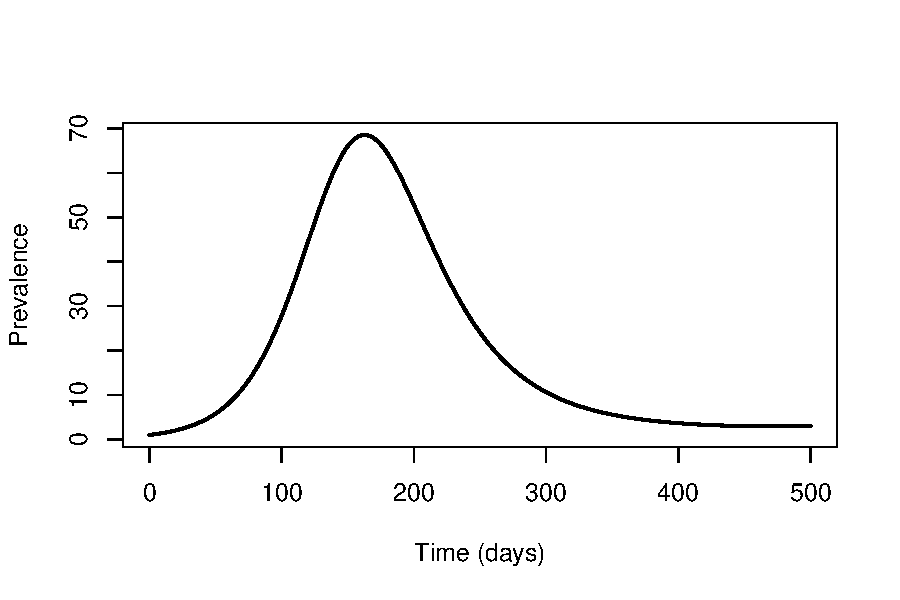
\includegraphics[width=\textwidth]{FIGS/L13-SIRS_one_sim_prevalence-1.pdf}
  \end{center}
\end{frame}

\begin{frame}{I just did ...}

What I advise not to do: illustrate a mathematical result without adding anything to the result itself
\vfill
Let us make things a bit better. See the \href{https://raw.githubusercontent.com/julien-arino/3MC-2023-12-Arba-Minch/main/CODE/ODE_SIS_multiple_solutions.R}{code}
\end{frame}



\begin{frame}{}
  \begin{center}
    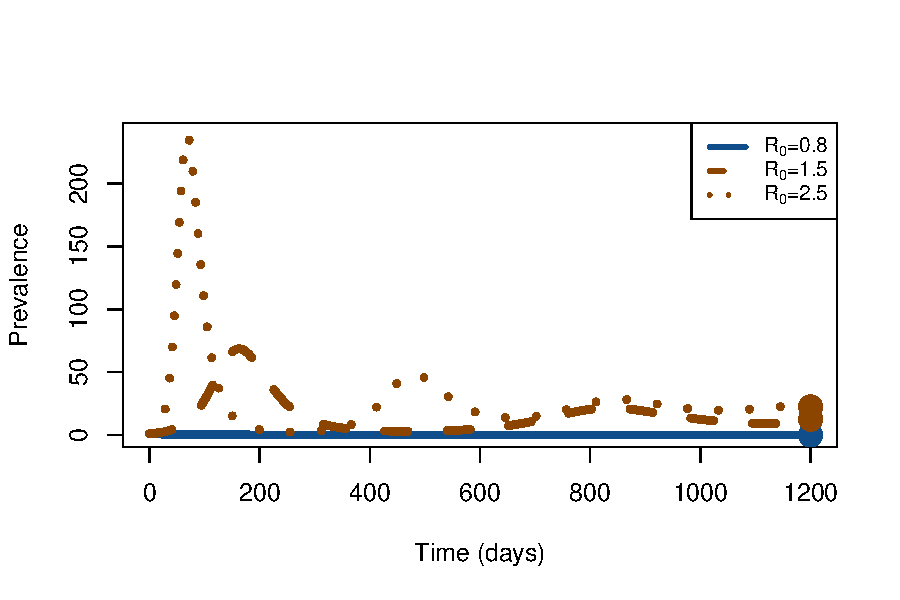
\includegraphics[width=\textwidth]{FIGS/L13-SIRS_3_sims_prevalence-1.pdf}
  \end{center}
\end{frame}

\begin{frame}
We could continue, but with a model this simple, there is little  more to do: the 3 parameters of the system are combined within $\R_0$ and the latter summarises the dynamics well
\vfill
We are going to show something important: the bifurcation diagram
\vfill
We saw that when $\R_0<1$, $I\to 0$, whereas when $\R_0>1$, $I\to (1-1/\R_0)N$. Let us represent this (\href{https://raw.githubusercontent.com/julien-arino/3MC-2023-12-Arba-Minch/main/CODE/SIS_PEI_vs_R0.R}{code})
\end{frame}



\begin{frame}
  \begin{center}
    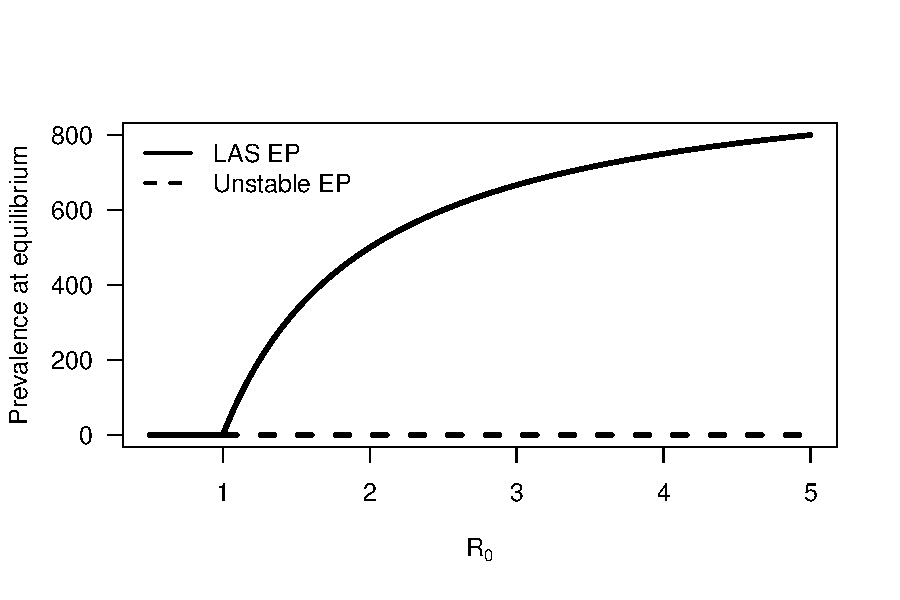
\includegraphics[width=\textwidth]{FIGS/L13-SIRS_bifurcation_R0-1.pdf}
  \end{center}
\end{frame}



%%%%%%%%%%%%%%%%%%%%%%%%%%%
%%%%%%%%%%%%%%%%%%%%%%%%%%%
\subsection{Herd immunity in the SIRS model}
\newSubSectionSlide{FIGS-slides-admin/Gemini_Generated_Image_vqpscpvqpscpvqps.jpeg}

\begin{frame}{An SIRS model with vaccination}
Take SIRS model \eqref{sys:SIRS} and assume the following
\vfill
\begin{itemize}
\item Vaccination takes newborn individuals and moves them directly into the removed compartment, without them becoming infected/infectious
\vfill
\item A fraction $p$ is vaccinated at birth
\end{itemize}
\end{frame}

\begin{frame}{The model}
\begin{minipage}{0.25\textwidth}
  \def\skip{*-1.5}
  \begin{tikzpicture}[scale=1, transform shape]
    %% Regular nodes
    \node [circle, fill=green!50, text=black] at (0,0) (S) {$S$};
    \node [circle, fill=red!90, text=black] at (0,1\skip) (I) {$I$};
    \node [circle, fill=blue!90, text=black] at (0,2\skip) (R) {$R$};
    %% Fake nodes for arrows
    \node [above=1cm of S] (birthS) {};
    \node [below=1cm of R] (birthR) {};
    \node [left=0.5cm of S] (dS) {};
    \node [left=0.5cm of I] (dI) {};
    \node [left=0.5cm of R] (dR) {};
    %% Flows
    \path [line, very thick, red] (birthS) to node [midway, right] (TextNode) {$(1-p)b$} (S);
    \path [line, very thick, red] (birthR) to node [midway, right] (TextNode) {$pb$} (R);
    \path [line, very thick] (S) to node [midway, above] (TextNode) {$dS$} (dS);
    \path [line, very thick] (I) to node [midway, above] (TextNode) {$dI$} (dI);
    \path [line, very thick] (R) to node [midway, above] (TextNode) {$dR$} (dR);
    \path [line, very thick] (S) to node [midway, right] (TextNode) {$\beta SI$} (I);
    \path [line, very thick] (I) to node [midway, right] (TextNode) {$\gamma I$} (R);
    \draw [>=latex,->, thick, rounded corners] (R) -- (0.8,2\skip) -- (0.8,0) node[midway, right] {$\nu R$} -- (S);
    \end{tikzpicture}    
\end{minipage}
\begin{minipage}{0.7\textwidth}
  \begin{subequations} \label{sys:SIR_vacc}
  \begin{align}
    S\pprime &= (1-p)b+\nu R-dS-\beta SI \label{sys:SIR_vacc_dS} \\
    I\pprime &= \beta SI-(d+\gamma) I \label{sys:SIR_vacc_dI} \\
    R\pprime &= bp+\gamma I-(d+\nu)R \label{sys:SIR_vacc_dR}
  \end{align}    
  \end{subequations}
  \vskip1cm
  Consider the initial value problem consisting in \eqref{sys:SIR_vacc} to which we adjoin initial conditions $S(0)=S_0\geq 0$, $I(0)=I_0\geq 0$ and $R(0)=R_0\geq 0$
  \vskip1cm
  Typically, we assume $N_0=S_0+I_0+R_0>0$ to avoid a trivial case
  \end{minipage}
\end{frame}

\begin{frame}{This modification doesn't change much}
Equation \eqref{eq:total_pop_general} for the total population is unchanged
\vfill
The Jacobian \eqref{eq:SIRS_Jacobian} at arbitrary point is also unchanged
\vfill 
The DFE is affected, though; as a consequence, so is the reproduction number
\end{frame}

\begin{frame}{The DFE for the SIRS vaccination model}
Considering \eqref{sys:SIR_vacc} at equilibrium and substituting $I^\star=0$ into this system gives
\begin{align*}
0 &= (1-p)b+\nu R^\star-dS^\star \\
0 &= bp-(d+\nu)R^\star
\end{align*}
which we rewrite as the linear system
\[
\begin{pmatrix}
d & -\nu \\ 0 & d+\nu
\end{pmatrix}
\begin{pmatrix}
S^\star \\ R^\star
\end{pmatrix}
=
\begin{pmatrix}
(1-p)b \\ bp
\end{pmatrix}
\]
Thus
\begin{align*}
\begin{pmatrix}
S^\star \\ R^\star
\end{pmatrix}
&= \frac{1}{d(d+\nu)}
\begin{pmatrix}
d+\nu & \nu \\ 0 & d
\end{pmatrix}
\begin{pmatrix}
(1-p)b \\ pb
\end{pmatrix} \\
&= \frac{1}{d(d+\nu)}
\begin{pmatrix}
(d+\nu)(1-p)b+pb\nu \\ pbd
\end{pmatrix}
\end{align*}
\end{frame}

\begin{frame}
As a consequence, the DFE takes the form
\begin{equation}\label{eq:SIRS_vacc_DFE}
\bE_0^v := (S^\star,I^\star,R^\star) =
\left(
\left(1-p+\frac{p\nu}{d+\nu}\right)N^\star,0,
\frac{pd}{d+\nu}N^\star
\right)
\end{equation}
\vfill
Substituting \eqref{eq:SIRS_vacc_DFE} into the eigenvalue that determines stability of the DFE, $\beta S^\star-(d+\gamma)$, we get
\begin{align*}
\beta S^\star-(d+\gamma)<0 &\iff
\frac\beta{d+\gamma} S^\star <1 \\
&\iff 
\frac\beta{d+\gamma}
\left(1-p+\frac{p\nu}{d+\nu}\right)N^\star<1
\end{align*}
So we define
\begin{equation}\label{eq:SIRS_vacc_R0}
\R_0^v =
\frac\beta{d+\gamma}
\left(1-p+\frac{p\nu}{d+\nu}\right)N^\star
\end{equation}
\end{frame}


\begin{frame}{Herd immunity}
  Therefore 
  \begin{itemize}
  \item $\R_0^{\textrm{v}}<\R_0$ if $p>0$
  \item To control the disease, $\R_{\text{v}}$ must take a value less than 1, i.e.,
  \begin{equation}
    \R_{\text{v}}<1 \iff p> 1-\frac{1}{\R_0}
  \end{equation}
  \end{itemize}
  \vfill
  By vaccinating a fraction $p>1-1/\R_0$ of newborns, we thus are in a situation where the disease is eventually eradicated
  \vfill
  This is \defword{herd immunity} (\emph{bis repetita})
\end{frame}

%%%%%%%%%%%%%%
%%%%%%%%%%%%%%
\subsection{SLIRS model with constant population}
\newSubSectionSlide{FIGS-slides-admin/Gemini_Generated_Image_vqpscpvqpscpvqps.jpeg}

\frame{\frametitle{Incubation periods}
\begin{itemize}
\item SIS and SIR: progression from S to I is instantaneous
\vfill
\item Several incubation periods:
\end{itemize}
\begin{center}
\begin{tabular}{l|l}
Disease & Incubation period \\
\hline
Yersinia Pestis & 2-6 days \\
Ebola haemorrhagic fever (HF) & 2-21 days \\
Marburg HF & 5-10 days \\
Lassa fever & 1-3 weeks \\
Tse-tse & weeks--months \\
HIV/AIDS & months--years
\end{tabular}
\end{center}
}

\frame{\frametitle{Hypotheses}
\begin{itemize}
\item There is demography
\item New individuals are born at a constant rate $b$
\item
There is no vertical transmssion: all ``newborns'' are susceptible
\item The disease is non lethal, it causes no additional mortality
\item New infections occur at the rate $f(S,I,N)$
\item There is a period of incubation for the disease
\item There is a period of time after recovery during which the disease confers immunity to reinfection (immune period)
\end{itemize} 
}

\frame{\frametitle{SLIRS}
\begin{minipage}{0.2\textwidth}
  \def\skip{*-1.5}
  \begin{tikzpicture}[scale=1, transform shape]
    %% Regular nodes
    \node [circle, fill=green!50, text=black] at (0,0) (S) {$S$};
    \node [circle, fill=red!50, text=black] at (0,1\skip) (L) {$L$};
    \node [circle, fill=red!90, text=black] at (0,2\skip) (I) {$I$};
    \node [circle, fill=blue!50, text=black] at (0,3\skip) (R) {$R$};
    %% Fake nodes for arrows
    \node [above=0.75cm of S] (birth) {};
    \node [left=0.5cm of S] (dS) {};
    \node [left=0.5cm of L] (dL) {};
    \node [left=0.5cm of I] (dI) {};
    \node [left=0.5cm of R] (dR) {};
    %% Flows (demography)
    \path [line, very thick] (birth) to node [midway, left] (TextNode) {$b$} (S);
    \path [line, very thick] (S) to node [midway, above] (TextNode) {$dS$} (dS);
    \path [line, very thick] (L) to node [midway, below] (TextNode) {$dL$} (dL);
    \path [line, very thick] (I) to node [midway, below] (TextNode) {$dI$} (dI);
    \path [line, very thick] (R) to node [midway, below] (TextNode) {$dR$} (dR);
    %% Flows (demography)
    \path [line, very thick] (S) to node [midway, left] (TextNode) {$f(S,I,N)$} (L);
    \path [line, very thick] (L) to node [midway, left] (TextNode) {$\varepsilon L$} (I);
    \path [line, very thick] (I) to node [midway, left] (TextNode) {$\gamma I$} (R);
    \draw [>=latex,->, thick, rounded corners] (R) -- (0.75,3\skip) -- (0.75,0) node[midway,above,sloped] {$\nu R$} -- (S);
  \end{tikzpicture}    
\end{minipage}
\quad
\begin{minipage}{0.7\textwidth}
The model is as follows:
\begin{subequations}\label{sys:SLIRS}
\begin{align}
S\pprime &= b+\nu R-dS-f(S,I,N) \label{sys:SLIRS_dS} \\
L\pprime &= f(S,I,N) -(d+\varepsilon)L \label{sys:SLIRS_dL} \\
I\pprime &= \varepsilon L -(d+\gamma)I \label{sys:SLIRS_dI} \\
R\pprime &= \gamma I-(d+\nu)R \label{sys:SLIRS_dR} 
\end{align}
\end{subequations}
\vfill
Meaning of the parameters:
\begin{itemize}
\item $1/\varepsilon$ average duration of the incubation period
\item $1/\gamma$ average duration of infectious period
\item $1/\nu$ average duration of immune period
\end{itemize}
\end{minipage}
}



%%%%%%%%%%%%%%%%%%%%%%%
%%%%%%%%%%%%%%%%%%%%%%%
\subsection{Computing $\R_0$ more efficiently}
\newSubSectionSlide{FIGS-slides-admin/Gemini_Generated_Image_vqpscpvqpscpvqps.jpeg}

\maxFrameImage{FIGS/PvdDWatmough2002.png}
\nocite{VdDWatmough2002}


\frame{\frametitle{The basic reproduction number $\R_0$}
Used frequently in epidemiology (not only math epi)
\begin{definition}[$R_0$]
The basic reproduction number $\R_0$ is the average number of secondary cases generated by the introduction of an infectious individual in a wholly susceptible population
\end{definition}
\begin{itemize}
\item If $\R_0<1$, then on average, each infectious individual infects less than one other person, so the epidemic has chances of dying out
\item If $\R_0>1$, then on average, each infectious individual infects more than one other person and the disease can become established in the population (or there will be a major epidemic)
\end{itemize}
}

\frame{\frametitle{Computation of $\R_0$}
Mathematically, $\R_0$ is a bifurcation parameter aggregating some of the model parameters and such that the disease free equilibrium (DFE) loses its local asymptotic stability when $\R_0=1$ is crossed from left to right
\vfill
\begin{itemize}
\item
As a consequence, $\R_0$ is found by considering the spectrum of the Jacobian matrix of the system evaluated at the DFE
\vfill
\item
The matrix quickly becomes hard to deal with (size and absence of ``pattern'') and the form obtained is not unique, which is annoying when trying to interpret $\R_0$
\end{itemize}
}

\begin{frame}{Preliminary setup of PvdD \& Watmough 2002}
$x=(x_1,\ldots,x_n)^T$, $x_i\geq 0$, with the first $m<n$ compartments the infected ones
\vfill
$X_s$ the set of all disease free states: 
\[
X_s=\{x\geq 0| x_i=0, i=1,\ldots,m\}
\]
\vfill
Distinguish new infections from all other changes in population
\begin{itemize}
\item $F_i(x)$ rate of appearance of new infections in compartment $i$
\item $V_i^+(x)$ rate of transfer of individuals into compartment $i$ by all other means
\item $V_i^-(x)$ rate of transfer of individuals out of compartment $i$
\end{itemize}
\vfill
Assume each function continuously differentiable at least twice in each variable
\vfill
\[
x_i' = f_i(x)=F_i(x)-V_i(x),\quad i=1,\ldots,n
\]
where $V_i=V_i^--V_i^+$
\end{frame}

\begin{frame}{Some assumptions}
\bbullet\textbf{(A1)}
If $x\geq 0$, then $F_i,V_i^+,V_i^-\geq 0$ for $i=1,\ldots,n$
\vfill
Since each function represents a directed transfer of individuals, all are non-negative
\vfill
\bbullet\textbf{(A2)} 
If $x_i=0$ then $V_i^-=0$. In particular, if $x\in X_s$, then $V_i^-=0$ for $i=1,\ldots,m$
\vfill
If a compartment is empty, there can be no transfer of individuals out of the compartment by death, infection, nor any other means
\end{frame}

\begin{frame}
\bbullet \textbf{(A3)} $F_i=0$ if $i>m$
\vfill
The incidence of infection for uninfected compartments is zero
\vfill
\bbullet \textbf{A4} If $x\in X_s$ then $F_i(x)=0$ and $V_i^+(x)=0$ for $i=1,\ldots,m$
\vfill
Assume that if the population is free of disease then the population will remain free of disease; i.e., there is no (density independent) immigration of infectives
\end{frame}

\begin{frame}{One last assumption for the road}
Let $x_0$ be a DFE of the system, i.e., a (locally asymptotically) stable equilibrium solution of the disease free model, i.e., the system restricted to $X_s$. We need not assume that the model has a unique DFE
\vfill
Let $Df(x_0)$ be the Jacobian matrix $[\partial f_i/\partial x_j]$. Some derivatives are one sided, since $x_0$ is on the domain boundary
\vfill
\textbf{(A5)} If $F(x)$ is set to zero, then all eigenvalues of $Df(x_0)$ have negative real parts
\vfill
Note: if the method ever fails to work, it is usually with (A5) that lies the problem
\end{frame}

\begin{frame}{Stability of the DFE as function of $\mathcal{R}_0$}
\begin{theorem}\label{th:R0_VdDW}
Suppose the DFE exists. Let then
\[
\mathcal{R}_0=\rho(FV^{-1})
\]
with matrices $F$ and $V$ obtained as indicated. Assume conditions (A1) through (A5) hold. Then
\begin{itemize}
\item if $\mathcal{R}_0<1$, then the DFE is LAS
\item if $\mathcal{R}_0>1$, the DFE is unstable
\end{itemize}
\end{theorem}
\vfill
Important to stress \emph{local} nature of stability that is deduced from this result. We will see later that even when $\mathcal{R}_0<1$, there can be several positive equilibria
\end{frame}

\begin{frame}{Direction of the bifurcation at $\mathcal{R}_0=1$}
$\mu$ bifurcation parameter s.t. $\mathcal{R}_0<1$ for $\mu<0$ and $\mathcal{R}_0>1$ for $\mu>0$ and $x_0$ DFE for all values of $\mu$ and consider the system
\begin{equation}
\label{eq:sys_PvdDW}
x'=f(x,\mu)
\end{equation}
\vfill
Write 
\[
D_xf(x_0,0)=
\left. 
  D(\mathcal{F}(x_0)-\mathcal{V}(x_0))
\right|_{\mathcal{R}_0=1}
\]
as block matrix
\[
D\mathcal{F}(x_0)
=\begin{pmatrix}
F & 0 \\ 0 & 0
\end{pmatrix},
\quad
D\mathcal{V}(x_0)
=\begin{pmatrix}
V & 0 \\ J_3 & J_4
\end{pmatrix}
\]
\end{frame}

\begin{frame}
Write $[\alpha_{\ell k}]$, $\ell=m+1,\ldots,n$, $k=1,\ldots,m$ the $(\ell-m,k)$ entry of $-J_4^{-1}J_3$ and let $v$ and $w$ be left and right eigenvectors of $D_xf(x_0,0)$ s.t. $vw=1$
\vfill
Let
\begin{equation}
\label{eq:PvdDW_a}
a =\sum_{i,j,k=1}^m
v_iw_jw_k
\left(
\frac 12 
\frac{\partial^2f_i}{\partial x_j\partial x_k}(x_0,0)
+\sum_{\ell=m+1}^n
\alpha_{\ell k}
\frac{\partial^2f_i}{\partial x_j\partial x_\ell}(x_0,0)
\right)
\end{equation}
\vfill
\begin{equation}
\label{eq:PvdDW_b}
b
=vD_{x\mu}f(x_0,0)w
=\sum_{i,j=1}^n v_iw_j
\frac{\partial^2f_i}{\partial x_j\partial\mu}
(x_0,0)
\end{equation}
\end{frame}

\begin{frame}
\begin{theorem}
Consider model $\eqref{eq:sys_PvdDW}$ with $f(x,\mu)$ satisfying conditions (A1)–(A5) and $\mu$ as described above
\vskip1cm
Assume that the zero eigenvalue of $D_xf(x_0,0)$ is simple
\vskip1cm
Define $a$ and $b$ by $\eqref{eq:PvdDW_a}$ and $\eqref{eq:PvdDW_b}$; assume that $b\neq 0$. Then $\exists\delta > 0$ s.t.
\begin{itemize}
\item if $a < 0$, then there are LAS endemic equilibria near $x_0$ for $0 < \mu < \delta$
\item if $a > 0$, then there are unstable endemic equilibria near $x_0$ for $-\delta < \mu < 0$
\end{itemize}
\end{theorem}
\end{frame}


\frame{\frametitle{Example of the SLIRS model \eqref{sys:SLIRS}}
Variation of the infected variables in \eqref{sys:SLIRS} are described by
\begin{align*}
L\pprime &= f(S,I,N)-(\varepsilon+d) L \\
I\pprime &= \varepsilon L -(d+\gamma) I
\end{align*}
Write
\begin{equation}
\I\pprime = 
\left(
\begin{matrix}
L \\
I
\end{matrix}
\right)'
=\left(
\begin{matrix}
f(S,I,N) \\
0
\end{matrix}
\right)
-
\left(
\begin{matrix}
(\varepsilon+d) L \\
(d+\gamma) I-\varepsilon L
\end{matrix}
\right)=:\mathcal{F}-\mathcal{V}
\end{equation}
}


\frame{
Denote
\[
f_L^{\,\star}:=
\left.\frac{\partial}{\partial L}f
\right|_{(S,I,R)=\bE_0}
\quad\quad 
f_I^{\,\star}:=
\left.\frac{\partial}{\partial I}f
\right|_{(S,I,R)=\bE_0}
\]
the values of the partials of the incidence function at the DFE $\bE_0$
\vfill
Compute the Jacobian matrices of vectors $\F$ and $\V$ at the DFE $\bE_0$
\begin{equation}
F=\left(
\begin{matrix}
f_L^{\,\star} & f_I^{\,\star} \\
0 & 0
\end{matrix}
\right)
\quad\text{and}\quad
V=\left(
\begin{matrix}
\varepsilon+d & 0 \\
-\varepsilon & d+\gamma
\end{matrix}
\right)
\end{equation}
}

\frame{
Thus
\[
V^{-1}=\frac{1}{(d+\varepsilon)(d+\gamma)}
\left(
\begin{matrix}
d+\gamma & 0 \\
\varepsilon & d+\varepsilon
\end{matrix}
\right)
\]
\vfill
Also, in the case $N$ is constant, $\partial f/\partial L=0$ and thus
\[
FV^{-1}=\frac{f_I^{\,\star}}
{(d+\varepsilon)(d+\gamma)}
\left(
\begin{matrix}
\varepsilon 
& d+\varepsilon  \\
0 & 0
\end{matrix}
\right)
\]
\vfill
As a consequence,
\[
\R_0=\varepsilon
\frac{f_I^{\,\star}}
{(d+\varepsilon)(d+\gamma)}
\]
}


\frame{
\begin{theorem}\label{th:R0_SEIRS}
Let
\begin{equation}\label{eq:R0_SEIRS}
\R_0=
\frac{\varepsilon f_I^{\,\star}}
{(d+\varepsilon)(d+\gamma)}
\end{equation}
Then
\begin{itemize}
\item if $\R_0<1$, the DFE is LAS
\item if $\R_0>1$, the DFE is unstable
\end{itemize}
\end{theorem}
\vfill
It is important here to stress that the result we obtain concerns the \textbf{local} asymptotic stability. We see later that even when $\R_0<1$, there can be several locally asymptotically stable equilibria
}


\frame{\frametitle{Application}
The DFE is
\[
(\bar S,\bar L,\bar I,\bar R)=(N,0,0,0)
\]
\begin{itemize}
\item Mass action incidence (frequency-dependent contacts):
 \[
f_I^{\,\star}=\beta\bar S \Rightarrow\R_0 =
\frac{\epsilon\beta N}{(\epsilon+d)(\gamma+d)} 
\]
\item Standard incidence (proportion-dependent contacts):
\[
f_I^{\,\star}=\frac{\beta\bar S}{N}
\Rightarrow\R_0 = \frac{\epsilon\beta}{(\epsilon+d)(\gamma+d)}
\]
\end{itemize}
}


\frame{\frametitle{Links between SLIRS-type models}
{ %\footnotesize
\begin{align*}
S\pprime&=b+\nu R-dS-f(S,I,N) \\
L\pprime&=f(S,I,N)-(d+\varepsilon) L \\
I\pprime&=\varepsilon L-(d+\gamma)I \\
R\pprime&=\gamma I-(d+\nu)R
\end{align*}}
\begin{center}
\begin{tabular}{c|l}
\hline
SLIR & SLIRS where $\nu=0$ \\
SLIS & Limit of SLIRS when $\nu\to\infty$ \\
SLI & SLIR where $\gamma=0$ \\
SIRS & Limit of SLIRS when $\varepsilon\to\infty$ \\
SIR & SIRS where $\nu=0$ \\
SIS & Limit of SIRS when $\nu\to\infty$ \\
& Limit SLIS when $\varepsilon\to\infty$ \\
SI & SIS where $\nu=0$ 
\end{tabular}
\end{center}
}

\frame{\frametitle{Values of $\R_0$}
$(\bar S,\bar I,\bar N)$ values of $S,I$ and $N$ at DFE. Denote $\bar f_I=\partial f/\partial I(\bar S,\bar I,\bar N)$.
\begin{center}
\begin{tabular}{c|c}
\hline
SLIRS & 
$\frac{\varepsilon\bar f_I}{(d+\varepsilon)(d+\gamma)}$ \\
SLIR & 
$\frac{\varepsilon\bar f_I}{(d+\varepsilon)(d+\gamma)}$ \\
SLIS & 
$\frac{\varepsilon\bar f_I}{(d+\varepsilon)(d+\gamma)}$ \\
SLI & 
$\frac{\varepsilon\bar f_I}{(d+\varepsilon)(d+\gamma)}$ \\
& \\
SIRS & 
$\frac{\varepsilon\bar f_I}{d+\gamma}$ \\
SIR & $\frac{\bar f_I}{d+\gamma}$ \\
SIS & $\frac{\bar f_I}{d+\gamma}$ \\
SI & $ \frac{\bar f_I}{d+\gamma}$ 
\end{tabular}
\end{center}
}


%%%%%%%%%%%%%%%%%%%%%%%
%%%%%%%%%%%%%%%%%%%%%%%
\subsection{A better vaccination model?}
\newSubSectionSlide{FIGS-slides-admin/Gemini_Generated_Image_vqpscpvqpscpvqps.jpeg}

\maxFrameImage{FIGS/ArinoMccluskeyPvdD.png}
\nocite{ArinoMccluskeyVdD2003}

\begin{frame}{SLIRS with vaccination}
\centering
  \def\skip{*2.5}
  \begin{tikzpicture}[scale=1.5, transform shape]
    %% Regular nodes
    \node [circle, fill=green!50, text=black] at (0,0) (S) {$S$};
    \node [circle, fill=red!90, text=black] at (1\skip,0) (I) {$I$};
    \node [circle, fill=blue!50, text=black] at (2\skip,0) (R) {$R$};
    \node [circle, fill=red!50, text=black] at (0.5\skip,-1\skip) (V) {$V$};
    %% Fake nodes for arrows
    \node [left=0.75cm of S] (birth) {};
    \node [below=0.5cm of S] (dS) {};
    \node [below=0.5cm of I] (dI) {};
    \node [below=0.5cm of R] (dR) {};
    \node [below=0.5cm of V] (dV) {};
    %% Flows (demography)
    \path [line, very thick] (birth) to node [midway, above] (TextNode) {$b$} (S);
    \path [line, very thick] (S) to node [midway, left] (TextNode) {$dS$} (dS);
    \path [line, very thick] (I) to node [midway, right] (TextNode) {$dI$} (dI);
    \path [line, very thick] (R) to node [midway, left] (TextNode) {$dR$} (dR);
    \path [line, very thick] (V) to node [midway, left] (TextNode) {$dV$} (dV);
    %% Flows
    \path [line, very thick] (S) to node [midway, above] (TextNode) {$\beta SI/N$} (I);
    \path [line, very thick, bend left=10] (S) to node [near start, right] (TextNode) {$\phi S$} (V);
    \path [line, very thick, bend left=10] (V) to node [near start, left] (TextNode) {$\varphi V$} (S);
    \path [line, very thick] (V) to node [midway, above, sloped] (TextNode) {$\sigma\beta VI/N$} (I);
    \path [line, very thick] (I) to node [midway, above] (TextNode) {$\gamma I$} (R);
    \draw [>=latex,->, thick, rounded corners] (R) -- (2\skip,0.75) -- (0,0.75) node[midway,above,sloped] {$\nu R$} -- (S);
  \end{tikzpicture}    
\end{frame}

\begin{frame}{The usual situation}
\centering
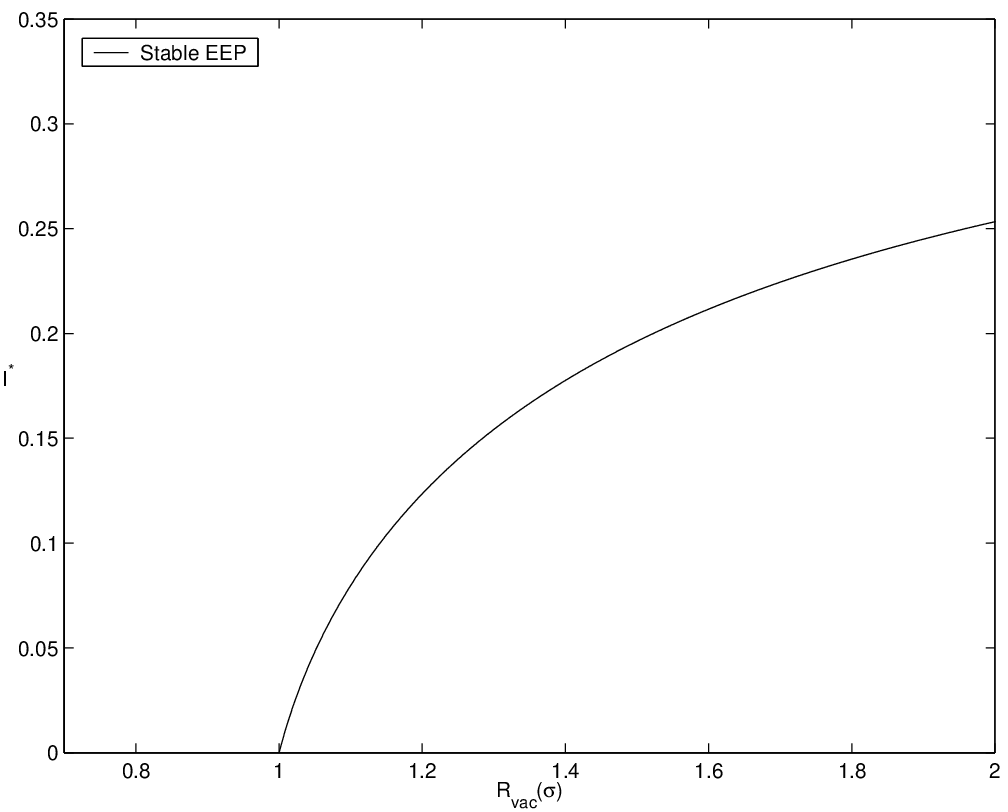
\includegraphics[width=0.7\textwidth]{FIGS/SIRV_bif_forward}
\end{frame}

\begin{frame}{What can happen with vaccination -- Backward bifurcation}
\centering
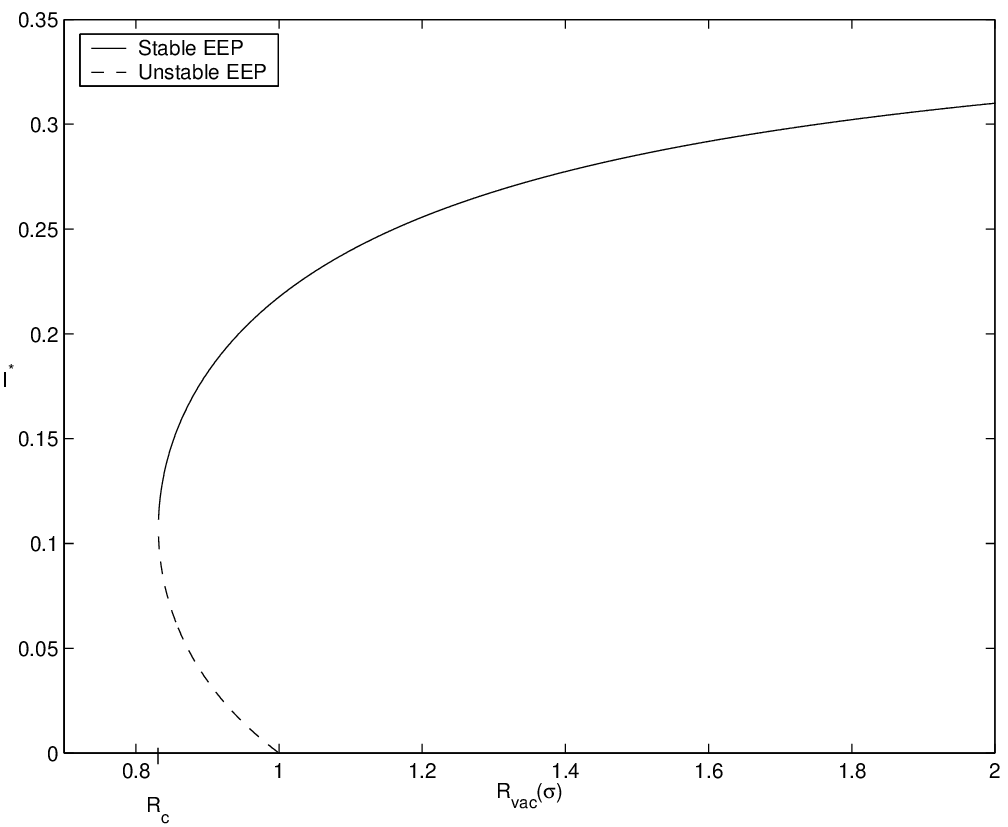
\includegraphics[width=0.7\textwidth]{FIGS/SIRV_bif_backward}
\end{frame}


%%%%%%%%%%%%%%%%%%%%
%%%%%%%%%%%%%%%%%%%%
%%%%%%%%%%%%%%%%%%%%
%%%%%%%%%%%%%%%%%%%%
\section{What if there's another guest at the party?}
\newSectionSlide{FIGS-slides-admin/Gemini_Generated_Image_4ls25f4ls25f4ls2.jpeg}

%%%%%%%%%%%%%%%%%%%%
%%%%%%%%%%%%%%%%%%%%
\subsection{Two Ross-Macdonald-type models}
\newSubSectionSlide{FIGS-slides-admin/Gemini_Generated_Image_4ls25f4ls25f4ls2.jpeg}
\begin{frame}
See, e.g., Simoy \& Aparicio, \href{https://doi.org/10.1016/j.actatropica.2020.105452}{Ross-Macdonald models: Which one should we use?}, \emph{Acta Tropica} (2020)
\vfill
Ross introduced the model in 1911. Later ``tweaked'' by Macdonald to include mosquito latency period
\vfill
Here, I show a version in the paper cited, with some notation changed
\end{frame}

\begin{frame}
\centering
\resizebox{\textwidth}{!}{
  \def\horskip{*2}
  \def\verskip{*2}
  \begin{tikzpicture}[%transform canvas={scale=1.3},
      auto,
      cloud/.style={minimum width={width("N-1")+2pt},
      draw, 
      ellipse,
      fill=gray!20}]
    %% Hosts
    \node [cloud, fill=green!50] at (0,0) (SH) {$S_H$};
    \node [cloud, fill=red!50] at (1\horskip,0) (IH) {$I_H$};
    \node [cloud, fill=blue!50] at (2\horskip,0) (RH) {$R_H$};
    %% Vectors
    \node [cloud, fill=green!50] at (0,-1\verskip) (SV) {$S_V$};
    \node [cloud, fill=red!50] at (1\horskip,-1\verskip) (IV) {$I_V$};
    %% Births
    \node [left=0.75cm of SH] (birthH) {};
    \node [left=0.75cm of SV] (birthV) {};
    %% Deaths
    \node [below=0.25\verskip of SH] (dSH) {};
    \node [below=0.25\verskip of IH] (dIH) {};
    \node [below=0.25\verskip of RH] (dRH) {};
    \node [below=0.25\verskip of SV] (dSV) {};
    \node [below=0.25\verskip of IV] (dIV) {};
    %%
    \path [line, very thick] (SH) to node [midway,above,sloped] (TextNode) {$\beta_HI_V\frac{S_H}{H}$} (IH);
    \path [line, very thick] (IH) to node [midway,above,sloped] (TextNode) {$\gamma_H I_H$} (RH);
    \path [line, very thick] (SV) to node [midway,below,sloped] (TextNode) {$\beta_VS_V\frac{I_H}{H}$} (IV);
    \path [line, dotted, very thick] (IV) to node [midway,below,sloped] (TextNode) {} (SH);
    \path [line, dotted, very thick] (IH) to node [midway,above,sloped] (TextNode) {} (SV);
    %% Demography
    \path [line, very thick] (birthH) to node [midway,above] (TextNode) {$b_H$} (SH);
    \path [line, very thick] (birthV) to node [midway,above] (TextNode) {$b_V$} (SV);
    \path [line, very thick] (SH) to node [near end,left] (TextNode) {$d_HS_H$} (dSH);
    \path [line, very thick] (IH) to node [near end,right] (TextNode) {$d_HI_H$} (dIH);
    \path [line, very thick] (RH) to node [near end,right] (TextNode) {$d_HR_H$} (dRH);
    \path [line, very thick] (SV) to node [near end,left] (TextNode) {$d_VS_V$} (dSV);
    \path [line, very thick] (IV) to node [near end,right] (TextNode) {$d_VI_V$} (dIV);
  \end{tikzpicture}
}
\end{frame}

\begin{frame}{Reproduction number}
\begin{equation}\label{eq:vector_host_1}
\R_0 =
\frac{\beta_H\beta_V}{(\gamma_H+\gamma_V)d_V}\
\frac{V^\star}{H^\star}
\end{equation}
where $H^\star$ and $V^\star$ are the total host and vector populations, respectively
\end{frame}


\begin{frame}
\centering
\resizebox{\textwidth}{!}{
  \def\horskip{*2}
  \def\verskip{*2}
  \begin{tikzpicture}[%transform canvas={scale=1.3},
      auto,
      cloud/.style={minimum width={width("N-1")+2pt},
      draw, 
      ellipse,
      fill=gray!20}]
    %% Hosts
    \node [cloud, fill=green!50] at (0,0) (SH) {$S_H$};
    \node [cloud, fill=red!10] at (1\horskip,0) (LH) {$L_H$};
    \node [cloud, fill=red!50] at (2\horskip,0) (IH) {$I_H$};
    \node [cloud, fill=blue!50] at (3\horskip,0) (RH) {$R_H$};
    %% Vectors
    \node [cloud, fill=green!50] at (0,-1\verskip) (SV) {$S_V$};
    \node [cloud, fill=red!10] at (1\horskip,-1\verskip) (LV) {$L_V$};
    \node [cloud, fill=red!50] at (2\horskip,-1\verskip) (IV) {$I_V$};
    %% Births
    \node [left=0.75cm of SH] (birthH) {};
    \node [left=0.75cm of SV] (birthV) {};
    %% Deaths
    \node [above=0.5\verskip of SH] (dSH) {};
    \node [above=0.5\verskip of LH] (dLH) {};
    \node [above=0.5\verskip of IH] (dIH) {};
    \node [above=0.5\verskip of RH] (dRH) {};
    \node [below=0.5\verskip of SV] (dSV) {};
    \node [below=0.5\verskip of LV] (dLV) {};
    \node [below=0.5\verskip of IV] (dIV) {};
    %%
    \path [line, very thick] (SH) to node [midway,above,sloped] (TextNode) {$\beta_HI_V\frac{S_H}{H}$} (LH);
    \path [line, very thick] (LH) to node [midway,above,sloped] (TextNode) {$\varepsilon_H L_H$} (IH);
    \path [line, very thick] (IH) to node [midway,above,sloped] (TextNode) {$\gamma_H I_H$} (RH);
    \path [line, very thick] (SV) to node [midway,below,sloped] (TextNode) {$\beta_VS_V\frac{I_H}{H}$} (LV);
    \path [line, very thick] (LV) to node [midway,below,sloped] (TextNode) {$\varepsilon_V L_V$} (IV);
    \path [line, dotted, very thick] (IV) to node [midway,below,sloped] (TextNode) {} (SH);
    \path [line, dotted, very thick] (IH) to node [midway,above,sloped] (TextNode) {} (SV);
    %% Demography
    \path [line, very thick] (birthH) to node [midway,above] (TextNode) {$b_H$} (SH);
    \path [line, very thick] (birthV) to node [midway,above] (TextNode) {$b_V$} (SV);
    \path [line, very thick] (SH) to node [near end,right] (TextNode) {$d_HS_H$} (dSH);
    \path [line, very thick] (LH) to node [near end,right] (TextNode) {$d_HL_H$} (dLH);
    \path [line, very thick] (IH) to node [near end,right] (TextNode) {$d_HI_H$} (dIH);
    \path [line, very thick] (RH) to node [near end,right] (TextNode) {$d_HR_H$} (dRH);
    \path [line, very thick] (SV) to node [near end,right] (TextNode) {$d_VS_V$} (dSV);
    \path [line, very thick] (LV) to node [near end,right] (TextNode) {$d_VL_V$} (dLV);
    \path [line, very thick] (IV) to node [near end,right] (TextNode) {$d_VI_V$} (dIV);
  \end{tikzpicture}
}
\end{frame}

\begin{frame}{Reproduction number}
\begin{equation}\label{eq:vector_host_2}
\R_0 =
\frac{\beta_H\beta_V}{(\gamma_H+\gamma_V)d_V}\
\frac{\varepsilon_V}{d_V+\varepsilon_V}\
\frac{\varepsilon_H}{d_H+\varepsilon_H}\
\frac{V^\star}{H^\star}
\end{equation}
where $H^\star$ and $V^\star$ are the total host and vector populations, respectively
\vfill
Here
\[
f_X = \frac{\varepsilon_X}{d_X+\varepsilon_X}
\]
are the fractions of latent individuals (of type $X=\{V,H\}$) who survive the latency period
\end{frame}


%%%%%%%%%%%%%%%%%%%%
%%%%%%%%%%%%%%%%%%%%
\subsection{A little complexification of Ross-Macdonald}
\newSubSectionSlide{FIGS-slides-admin/Gemini_Generated_Image_mco1ecmco1ecmco1.jpeg}

\begin{frame}{Recall this guy?}
\centering
\resizebox{\textwidth}{!}{
  \def\horskip{*2}
  \def\verskip{*2}
  \begin{tikzpicture}[%transform canvas={scale=1.3},
      auto,
      cloud/.style={minimum width={width("N-1")+2pt},
      draw, 
      ellipse,
      fill=gray!20}]
    %% Hosts
    \node [cloud, fill=green!50] at (0,0) (SH) {$S_H$};
    \node [cloud, fill=red!50] at (1\horskip,0) (IH) {$I_H$};
    \node [cloud, fill=blue!50] at (2\horskip,0) (RH) {$R_H$};
    %% Vectors
    \node [cloud, fill=green!50] at (0,-1\verskip) (SV) {$S_V$};
    \node [cloud, fill=red!50] at (1\horskip,-1\verskip) (IV) {$I_V$};
    %% Births
    \node [left=0.75cm of SH] (birthH) {};
    \node [left=0.75cm of SV] (birthV) {};
    %% Deaths
    \node [below=0.25\verskip of SH] (dSH) {};
    \node [below=0.25\verskip of IH] (dIH) {};
    \node [below=0.25\verskip of RH] (dRH) {};
    \node [below=0.25\verskip of SV] (dSV) {};
    \node [below=0.25\verskip of IV] (dIV) {};
    %%
    \path [line, very thick] (SH) to node [midway,above,sloped] (TextNode) {$\beta_HI_V\frac{S_H}{H}$} (IH);
    \path [line, very thick] (IH) to node [midway,above,sloped] (TextNode) {$\gamma_H I_H$} (RH);
    \path [line, very thick] (SV) to node [midway,below,sloped] (TextNode) {$\beta_VS_V\frac{I_H}{H}$} (IV);
    \path [line, dotted, very thick] (IV) to node [midway,below,sloped] (TextNode) {} (SH);
    \path [line, dotted, very thick] (IH) to node [midway,above,sloped] (TextNode) {} (SV);
    %% Demography
    \path [line, very thick] (birthH) to node [midway,above] (TextNode) {$b_H$} (SH);
    \path [line, very thick] (birthV) to node [midway,above] (TextNode) {$b_V$} (SV);
    \path [line, very thick] (SH) to node [near end,left] (TextNode) {$d_HS_H$} (dSH);
    \path [line, very thick] (IH) to node [near end,right] (TextNode) {$d_HI_H$} (dIH);
    \path [line, very thick] (RH) to node [near end,right] (TextNode) {$d_HR_H$} (dRH);
    \path [line, very thick] (SV) to node [near end,left] (TextNode) {$d_VS_V$} (dSV);
    \path [line, very thick] (IV) to node [near end,right] (TextNode) {$d_VI_V$} (dIV);
  \end{tikzpicture}
}
\end{frame}


\begin{frame}{Let us add a few arrows}
\centering
\resizebox{0.8\textwidth}{!}{
  \def\horskip{*2}
  \def\verskip{*2}
  \begin{tikzpicture}[%transform canvas={scale=1.3},
      auto,
      cloud/.style={minimum width={width("N-1")+2pt},
      draw, 
      ellipse,
      fill=gray!20}]
    %% Hosts
    \node [cloud, fill=green!50] at (0,0) (SH) {$S_H$};
    \node [cloud, fill=red!50] at (1\horskip,0) (IH) {$I_H$};
    \node [cloud, fill=blue!50] at (2\horskip,0) (RH) {$R_H$};
    %% Vectors
    \node [cloud, fill=green!50] at (0,-1\verskip) (SV) {$S_V$};
    \node [cloud, fill=red!50] at (1\horskip,-1\verskip) (IV) {$I_V$};
    %% Births
    \node [left=0.75cm of SH] (birthH) {};
    \node [left=0.75cm of SV] (birthV) {};
    %% Deaths
    \node [below=0.25\verskip of SH] (dSH) {};
    \node [below=0.25\verskip of IH] (dIH) {};
    \node [below=0.25\verskip of RH] (dRH) {};
    \node [below=0.25\verskip of SV] (dSV) {};
    \node [below=0.25\verskip of IV] (dIV) {};
    %%
    \path [line, very thick] (SH) to node [midway,above,sloped] (TextNode) {$\Phi_H$} (IH);
    \path [line, very thick] (IH) to node [midway,above,sloped] (TextNode) {$\gamma_H I_H$} (RH);
    \path [line, very thick] (SV) to node [midway,below,sloped] (TextNode) {$\Phi_V$} (IV);
    \path [line, dotted, very thick] (IV) to node [midway,below,sloped] (TextNode) {} (SH);
    \path [line, dotted, very thick] (IH) to node [midway,above,sloped] (TextNode) {} (SV);
    \draw [>=latex,->, thick, rounded corners] (IH) -- (1\horskip,0.75) -- (0,0.75) node[midway,above,sloped] {$\rho_H I_H$} -- (SH);
    \draw [>=latex,->, thick, rounded corners] (RH) -- (2\horskip,1.5) -- (-0.35,1.5) node[midway,above,sloped] {$\nu_H R_H$} -- (SH.north west);
    %% Demography
    \path [line, very thick] (birthH) to node [midway,above] (TextNode) {$b_H$} (SH);
    \path [line, very thick] (birthV) to node [midway,above] (TextNode) {$b_V$} (SV);
    \path [line, very thick] (SH) to node [near end,left] (TextNode) {$d_HS_H$} (dSH);
    \path [line, very thick] (IH) to node [near end,right] (TextNode) {$d_HI_H$} (dIH);
    \path [line, very thick] (RH) to node [near end,right] (TextNode) {$d_HR_H$} (dRH);
    \path [line, very thick] (SV) to node [near end,left] (TextNode) {$d_VS_V$} (dSV);
    \path [line, very thick] (IV) to node [near end,right] (TextNode) {$d_VI_V$} (dIV);
  \end{tikzpicture}
}
\end{frame}

\begin{frame}
Arino, Ducrot \& Zongo, \href{https://julien-arino.github.io/assets/pdf/papers/2012_ArinoDucrotZongo-JMB64.pdf}{A metapopulation model for malaria with transmission-blocking partial immunity in hosts}, Journal of Mathematical Biology (2012) \nocite{ArinoDucrotZongo2012}
\vfill
Incidence functions take the form
\[
\Phi_H = b_H(H,V)\sigma_{VH}\frac{I_V}{V}
\]
and 
\[
\Phi_V = b_V(H,V)\left(\sigma_{HV}\frac{I_H}{H}+\hat\sigma_{HV}\frac{R_H}{H}\right)
\]
where $b_{H}$ and $b_V$ are numbers per unit time of mosquito bites a human has and the number of humans a mosquito bites, respectively
\end{frame}

\begin{frame}{Parameters of the incidence function}
\begin{itemize}
\item $\sigma_{HV}$ probability of transmission of the parasite (in gametocyte form) from
an infectious human to a susceptible mosquito
\item $\hat\sigma_{HV}$ probability of transmission of the parasite (in gametocyte form) from
a semi-immune human to a susceptible mosquito
\item $\sigma_{VH}$ probability of transmission of the parasite (in sporozoite form) from
an infectious mosquito to a susceptible human
\end{itemize}
\vfill
Additional parameter that can be factored in (all per unit time)
\begin{itemize}
\item $a_H$ maximum number of mosquito bites a human can receive
\item $a_V$ number of times one mosquito would ``want to'' bite humans
\item $a$ average number of bites given to humans by each mosquito
\end{itemize}
\end{frame}

\begin{frame}{People to read for malaria models (IMOBO)}
See also the work of 
\vfill
\begin{itemize}
\item \href{https://scholar.google.com/citations?user=AwKMfZ8AAAAJ&hl=en}{Gideon Ngwa} at the University of Buea
\vfill
\item \href{https://scholar.google.ch/citations?user=BMiKO0UAAAAJ&hl=en}{Nakul Chitnis} at the Swiss Tropical and Public Health Institute
\end{itemize}
\vfill
Many others...
\end{frame}


\begin{frame}{More complex models may be needed for malaria}
Timing of processes is critical in malaria
\vfill
Plasmodium life cycle in the mosquito is commensurate with mosquito lifetime
\vfill
Need models that are able to account for that, because ODEs are not really good at this (see beginning of Stochastic systems lecture)
\vfill
Mathematics becomes more complicated
\end{frame}

%%%%%%%%%%%%%%%%%%%%
%%%%%%%%%%%%%%%%%%%%
\subsection{A model for cholera}
\newSubSectionSlide{FIGS-slides-admin/Gemini_Generated_Image_ql7xv9ql7xv9ql7x.png}

\maxFrameImage{FIGS/Codeco-BMB-cover}
\nocite{codecco2001endemic}

\begin{frame}{Code\c{c}o's model}
\begin{minipage}{0.49\textwidth}
\begin{center}
  \begin{tikzpicture}[scale=1.25, transform shape]
    \usetikzlibrary{calc} %% <- For coordinate calculation
    \node [circle, fill=green!50, text=black] (S) {$S$};
    \node [circle, right=1.5cm of S, fill=red!90, text=black] (I) {$I$};
    \node [circle, below=1.5cm of I, fill=blue!90, text=black] (B) {$B$};
    \coordinate[left=of S] (bS);
    \coordinate[above=of S] (dS);
    \coordinate[above=of I] (dI);
    \coordinate[left=of B] (bB);
    \coordinate[right=of B] (dB);
    %% Births and deaths
    \path [line, very thick] (bS) to node [midway, above] (TextNode) {$d_HH$} (S);
    \path [line, very thick] (S) to node [midway, right] (TextNode) {$d_HS$} (dS);
    \path [line, very thick] (I) to node [midway, right] (TextNode) {$\gamma I$} (dI);
    \path [line, very thick] (bB) to node [midway, above] (TextNode) {$b_BB$} (B);
    \path [line, very thick] (B) to node [midway, above] (TextNode) {$d_BB$} (dB);
    %% Flows
    \path [line, very thick] (S) to node [midway, above] (TextNode) {$\beta\frac{B}{K+B}S$} (I);
    \path [line, very thick, dashed] (I) to node [midway, right] (TextNode) {$\zeta I$} (B);
    \path [line, dotted] (B) to ($(S)!.5!(I)$);
  \end{tikzpicture}    
\end{center}
\end{minipage}
\begin{minipage}{0.49\textwidth}
\begin{subequations}
\label{sys:cholera-codeco}
\begin{align}
S' &= d_H(H-S)-\beta\frac{B}{K+B}S \\
I' &= \beta\frac{B}{K+B}S-\gamma I \\
B' &= (b_B-d_B)B+\zeta I
\end{align}
\end{subequations}
$K$ concentration of cholera in water giving 50\% chance of catching it
\end{minipage}
\vfill
Note that the dashed arrow from $I$ to $B$ is not a flow: individuals do not convert into \emph{vibrio cholerae}
\end{frame}

%%%%%%%%%%%%%%%%%%%%
%%%%%%%%%%%%%%%%%%%%
\subsection{A model for zoonotic transmission of waterborne disease}
\newSubSectionSlide{FIGS-slides-admin/Gemini_Generated_Image_vqpscpvqpscpvqps.jpeg}

\maxFrameImage{FIGS/Waters_etal-waterborne.png}
\nocite{waters2016zoonotic}

\begin{frame}{Zoonotic transmission of waterborne disease}
Zoonoses are animal diseases that are transmitted to humans
\vfill
Model here used for instance to model Giardia transmission from possums to humans
\end{frame}

\begin{frame}
  \begin{center}
    \def\vertskip{*2}
    \def\horzskip{*3}
    \begin{tikzpicture}[scale=1, transform shape]
      \node [rectangle, fill=gray!10, text=black] at (-1\horzskip,0\vertskip) (S_H) {Susceptible humans};
      \node [rectangle, fill=gray!10, text=black] at (1\horzskip,0\vertskip) (I_H) {Infectious humans};
      \node [rectangle, fill=gray!10, text=black] at (-1\horzskip,2\vertskip) (S_A) {Susceptible animals};
      \node [rectangle, fill=gray!10, text=black] at (1\horzskip,2\vertskip) (I_A) {Infectious animals};
      \node [rectangle, fill=gray!10, text=black] at (0\horzskip,1\vertskip) (W) {Live oo/cysts in water};
      %% Flows 
      \path [line, very thick] (S_H.south east) to node [midway, below] (TextNode) {P2P transmission} (I_H.south west);
      \path [line, dashed, very thick] (S_H.north east) to node [near end, above] (TextNode) {conversion of oo/cysts to infection} (I_H.north west);
      \path [line, very thick, bend left] (I_H) to node [midway, below] (TextNode) {recovery} (S_H);
      \path [line, very thick] (S_A.north east) to node [midway, above] (TextNode) {A2A transmission} (I_A.north west);
      \path [line, very thick] (I_A.south west) to node [midway, below] (TextNode) {recovery} (S_A.south east);
      %% Flows of W
      \path [line, dashed, very thick] (W) to node [midway, above] (TextNode) {Death of oo/cysts in water} (-2\horzskip,1\vertskip);
      \path [line, dashed, very thick] (W) to node [near start, left] (TextNode) {pick up rate} (0\horzskip,0.35\vertskip);
      \path [line, dashed, very thick] (I_A) to node [midway, below] (TextNode) {deposit rate} (W);
    \end{tikzpicture}    
  \end{center}  
\end{frame}

\begin{frame}
  \begin{center}
    \def\vertskip{*2}
    \def\horzskip{*2}
    \begin{tikzpicture}[scale=1.25, transform shape]
      \node [circle, fill=gray!10, text=black] at (-1\horzskip,0\vertskip) (S_H) {$S_H$};
      \node [circle, fill=gray!10, text=black] at (1\horzskip,0\vertskip) (I_H) {$I_H$};
      \node [circle, fill=gray!10, text=black] at (-1\horzskip,2\vertskip) (S_A) {$S_A$};
      \node [circle, fill=gray!10, text=black] at (1\horzskip,2\vertskip) (I_A) {$I_A$};
      \node [circle, fill=gray!10, text=black] at (0\horzskip,1\vertskip) (W) {$W$};
      %% Flows between
      \path [line, very thick] (S_H) to node [midway, below] (TextNode) {$\beta_H$} (I_H);
      \path [line, dashed, very thick, bend left] (S_H) to node [near end, above] (TextNode) {$\rho$} (I_H);
      \path [line, very thick, bend left] (I_H) to node [midway, below] (TextNode) {$\gamma_HI_H$} (S_H);
      \path [line, very thick, bend left] (S_A) to node [midway, above] (TextNode) {$\beta_A$} (I_A);
      \path [line, very thick, bend left] (I_A) to node [midway, above] (TextNode) {$\gamma_AI_A$} (S_A);
      %% Flows of W
      \path [line, dashed, very thick] (W) to node [midway, above] (TextNode) {$\mu W$} (-0.75\horzskip,1\vertskip);
      \path [line, dashed, very thick] (W) to node [near start, left] (TextNode) {$\eta$} (0\horzskip,0.35\vertskip);
      \path [line, dashed, very thick] (I_A) to node [midway, below, sloped] (TextNode) {$\alpha I_A$} (W);
    \end{tikzpicture}    
  \end{center}  
\end{frame}


\begin{frame}{The full model}
  \begin{subequations}
    \label{sys:WaterHamilton_etal}
    \begin{align}
      S_A\pprime &= -\beta_AS_AI_A+\gamma_AI_A \\
      I_A\pprime &= \beta_AS_AI_A-\gamma_AI_A \\
      W\pprime &= \alpha I_A-\eta W(S_H+I_H)-\mu W \\
      S_H\pprime &= -\rho\eta WS_H-\beta_HS_HI_H+\gamma_HI_H \\
      I_H\pprime &= \rho\eta WS_H+\beta_HS_HI_H-\gamma_HI_H 
    \end{align}
  \end{subequations}
  \vfill
  Considered with $N_A=S_A+I_A$ and $N_H=S_H+I_H$ constant
\end{frame}

\begin{frame}{Simplified model}
  Because $N_A$ and $N_H$ are constant, \eqref{sys:WaterHamilton_etal} can be simplified:
  \begin{subequations}
    \label{sys:WaterHamilton_etal_simplified}
    \begin{align}
      I_A\pprime &= \beta_AN_AI_A-\gamma_AI_A-\beta_AI_A^2 \\
      W\pprime &= \alpha I_A-\eta WN_H-\mu W \\
      I_H\pprime &= \rho\eta W(N_H-I_H)+\beta_HN_HI_H-\gamma_HI_H-\beta_HI_H^2 
    \end{align}
  \end{subequations}
  \vfill
  Three EP: DFE $(0,0,0)$; endemic disease in humans because of H2H transmission; endemic in both H and A because of W
\end{frame}


\begin{frame}
  Three EP: DFE $(0,0,0)$; endemic disease in humans because of H2H transmission; endemic in both H and A because of W
  \vfill
  Let
  \begin{equation}
    \R_{0A} = \frac{\beta_A}{\gamma_A}N_A\quad\text{and}\quad
    \R_{0H} = \frac{\beta_H}{\gamma_H}N_H
  \end{equation}
  \vfill
  \begin{itemize}
    \item DFE LAS if $\R_{0A}<1$ and $\R_{0H}<1$, unstable if $\R_{0A}>1$ or $\R_{0H}>1$
    \item If $\R_{0H}>1$ and $\R_{0A}<1$, \eqref{sys:WaterHamilton_etal_simplified} goes to EP with endemicity only in humans
    \item Endemic EP with both A and H requires $\R_{0A}>1$ and $\R_{0H}<1$
  \end{itemize}
  Note that proof is \textbf{not} global
\end{frame}

%%%%%%%%%%%%%%%%%%%%%%%%%%%
%%%%%%%%%%%%%%%%%%%%%%%%%%%
%%%%%%%%%%%%%%%%%%%%%%%%%%%
%%%%%%%%%%%%%%%%%%%%%%%%%%%
\section{Last remarks}
\newSectionSlide{FIGS-slides-admin/Gemini_Generated_Image_hz99k3hz99k3hz99.jpeg}

\begin{frame}{To simplify or not to simplify?}
\bbullet In the KMK epidemic model \eqref{sys:KMK} and the SIRS endemic model \eqref{sys:SIRS}, since the total population is constant or asymptotically constant, it is possible to omit one of the state variables since $N^\star=S+I+R$
\vfill
\bbullet We often use $R=N^\star-S-I$
\vfill
\bbullet This can greatly simplify some computations
\vfill
\bbullet Whether to do it or not is a matter of preference
\end{frame}

\begin{frame}{To normalise or not to normalise?}
\bbullet In the KMK epidemic model \eqref{sys:KMK} and the SIRS endemic model \eqref{sys:SIRS}, since the total population is constant or asymptotically constant, it is possible to normalise to $N=1$
\vfill
\bbullet This can greatly simplify some computations
\vfill
\bbullet However, I am not a big fan: it is important to always have the ``sizes'' of objects in mind
\vfill
\bbullet If you do normalise, at least for a paper destined to mathematical biology, always do a ``return to biology'', i.e., interpret your results in a biological light, which often implies to return to original values
\end{frame}

\begin{frame}{Where we are}
\bbullet An \emph{epidemic} SIR model (the KMK SIR) in which the presence or absence of an epidemic wave is characterised by the value of $\R_0$
\vfill
\bbullet The KMK SIR has explicit solutions (in some sense). \textbf{This is an exception!}
\vfill
\bbullet An \emph{endemic} SIRS model in which the threshold $\R_0=1$ is such that, when $\R_0<1$, the disease goes extinct, whereas when $\R_0>1$, the disease becomes established in the population
\vfill
\bbullet Some simple variations on these models
\vfill
\bbullet A few models for vector-borne or water-borne diseases
\end{frame}

%%%%%%%%%%%%%%%%%%%%%%%
%%%%%%%%%%%%%%%%%%%%%%%
%%%%%%%%%%%%%%%%%%%%%%%
%%%%%%%%%%%%%%%%%%%%%%%
\begin{frame}[fragile]\frametitle{\textsc{Can I have this wrapped up to go?}}
To finish, we use the command \code{purl} to generate an \code{R} file (\code{course-01-introduction-math-epi.R}) in the CODE directory with all the code chunks in this \code{Rnw} file
\vfill
\begin{knitrout}
\definecolor{shadecolor}{rgb}{0.969, 0.969, 0.969}\color{fgcolor}\begin{kframe}
\begin{alltt}
\hlcom{# From https://stackoverflow.com/questions/36868287/purl-within-knit-duplicate-label-error}
\hldef{rmd_chunks_to_r_temp} \hlkwb{<-} \hlkwa{function}\hldef{(}\hlkwc{file}\hldef{)\{}
  \hldef{callr}\hlopt{::}\hlkwd{r}\hldef{(}\hlkwa{function}\hldef{(}\hlkwc{file}\hldef{,} \hlkwc{temp}\hldef{)\{}
    \hldef{out_file} \hlkwb{=} \hlkwd{sprintf}\hldef{(}\hlsng{"../CODE/%s"}\hldef{,} \hlkwd{gsub}\hldef{(}\hlsng{".Rnw"}\hldef{,} \hlsng{".R"}\hldef{, file))}
    \hldef{knitr}\hlopt{::}\hlkwd{purl}\hldef{(file,} \hlkwc{output} \hldef{= out_file,} \hlkwc{documentation} \hldef{=} \hlnum{1}\hldef{)}
  \hldef{\},} \hlkwc{args} \hldef{=} \hlkwd{list}\hldef{(file))}
\hldef{\}}
\hlkwd{rmd_chunks_to_r_temp}\hldef{(}\hlsng{"L07-endemic-SIRS.Rnw"}\hldef{)}
\end{alltt}
\begin{verbatim}
## [1] "../CODE/L07-endemic-SIRS.R"
\end{verbatim}
\end{kframe}
\end{knitrout}
\end{frame}


\begin{frame}[allowframebreaks]{Bibliography}
\bibliographystyle{plain}
\bibliography{local-bibliography}
\end{frame}

\end{document}
